\chapter{Distributions as generalized functions}
\label{2011-m-ch:gf}

\section{Heuristically coping with discontinuities and singularities}

What follows are ``recipes'' and a ``cooking course'' for some ``dishes'' Heaviside, Dirac and others
have enjoyed ``eating,'' alas without being able to ``explain their digestion''
(cf. the citation by Heaviside on page \pageref{2013-m-ch-intro-cooking}).

Insofar theoretical physics is natural philosophy,
the question arises if ``measurable'' physical entities need to be ``smooth'' and ``continuous''~\cite{trench},
%\marginnote{{\tiny https://www.dpmms.cam.ac.uk/~wtg10/continuity.html}}
as ``nature abhors sudden discontinuities,''
or if we are willing to allow and conceptualize singularities of different sorts.
Other, entirely different,
scenarios are discrete,
computer-generated universes.
This little course is no place for preference and judgments regarding these matters.
Let me just point out that contemporary mathematical physics is not only leaning toward,
but appears to be deeply committed to discontinuities;
both in classical and quantized field theories dealing with
 ``point charges,''
as well as in general relativity,  the (nonquantized field theoretical)
geometrodynamics of gravitation,
dealing with singularities such as ``black holes'' or ``initial singularities'' of various sorts.

Discontinuities were introduced quite naturally as electromagnetic pulses,
which can, for instance, be described with the {\em Heaviside function}
$H(t)$ representing vanishing, zero field strength until time $t=0$, when suddenly a constant electrical field is
``switched on eternally.''
It is quite natural to ask what the derivative of the unit step function $H(t)$ might be.
---
At this point, the reader is kindly asked to stop reading for a moment and contemplate
on what kind of function that might be.

Heuristically, if we call this derivative the {\em (Dirac) delta function} $\delta$ defined by
$\delta (t)= \frac{d H(t)}{dt}$,
we can assure ourselves of two of its properties
(i) ``$\delta (t) =0$ for $t\neq 0$,''
as well as the antiderivative of the Heaviside function, yielding
(ii) ``$\int_{-\infty}^\infty \delta (t) dt  = \int_{-\infty}^\infty \frac{d H(t)}{dt} dt  =
H(\infty ) - H(-\infty ) = 1-0=1$.''

\marginnote{This heuristic definition of the Dirac delta function $\delta_y (x)= \delta (x,y)= \delta (x-y)$
with a discontinuity at $y$
is not unlike the discrete Kronecker symbol $\delta_{ij}$.
We may even define the Kronecker symbol $\delta_{ij}$
as the difference quotient of some ``discrete Heaviside function''
$H_{ij} =1$ for $i\ge j$, and $H_{i,j} =0$ else:
$\delta_{ij} = H_{ij} -H_{(i-1)j} = 1$ only for $i=j$; else it vanishes.}

Indeed, we could follow a pattern of ``growing discontinuity,''
reachable by ever higher and higher derivatives of the
absolute value (or modulus); that is, we shall pursue the path sketched by
$$
\vert x\vert
\stackrel{\frac{d}{dx}  }{  \longrightarrow}
\textrm{sgn}(x) ,\,
H(x)
\stackrel{\frac{d}{dx} }{ \longrightarrow}
\delta (x)
\stackrel{\frac{d^n}{dx^n} }{ \longrightarrow}
\delta^{(n)} (x)
.
$$



Objects like $\vert x\vert$,  $H(x)=\frac{1}{2}\left[ 1+\textrm{sgn}(x)\right]$ or $\delta (x)$ may be heuristically understandable
as ``functions'' not unlike
the regular analytic functions; alas
their $n$th derivatives cannot be straightforwardly defined.
In order to cope with a formally precise definition
and derivation of (infinite) pulse functions and to achieve this goal,
a theory of  {\em  generalized functions,}
or, used synonymously,
{\em distributions}
has been developed.
In what follows we shall
develop the theory of distributions;
always keeping in mind the assumptions
regarding (dis)continuities
that make necessary this part of the calculus.

The {\it Ansatz} pursued
\cite{richards_youn_1990}
will be to ``pair'' (that is, to multiply) these generalized functions $F$ with suitable ``good''
test functions $\varphi$,
and integrate over these functional pairs $F \varphi$.
Thereby we obtain a linear continuous functional
$F[\varphi]$,
also denoted by
$\langle F, \varphi \rangle $.
This strategy allows for the
``transference'' or ``shift'' of operations on, and transformations of, $F$
-- such as differentiations or Fourier transformations, but also multiplications with polynomials or other smooth functions --
to the test function $\varphi$ according to
{\em adjoint identities}
\index{adjoint identities}
\marginnote{See Sect. 2.3 in \cite{strichartz}}
\begin{equation}
\langle \textsf{\textbf{T}} F, \varphi \rangle
=
\langle F, \textsf{\textbf{S}} \varphi \rangle.
\end{equation}
For example,
for the $n$'th derivative,
\begin{equation}
\textsf{\textbf{S}} = (-1)^n \textsf{\textbf{T}} = (-1)^n \frac{d^{(n)}}{dx^{(n)}};
\end{equation}
and for the Fourier transformation,
\begin{equation}
\textsf{\textbf{S}} =   \textsf{\textbf{T}} = {\cal F} .
\end{equation}
For some (smooth) functional multiplier $g(x)\in C^\infty$ ,
\begin{equation}
\textsf{\textbf{S}} =   \textsf{\textbf{T}} = g(x) .
\label{2013-m-ch-di-multipl}
\end{equation}


One more issue is the problem of the meaning and existence of
{\em weak solutions} (also called   generalized solutions)
\index{weak solution}
of differential equations  for which, if interpreted in terms of regular functions,
the derivatives may not all exist.

{
\color{blue}
\bexample
Take, for example, the wave equation in one spatial dimension
$
\frac{\partial^2 }{\partial t^2} u(x,t)
=c^2
\frac{\partial^2 }{\partial x^2} u(x,t)
.
$
It has a  solution of the form \cite{Barut1990349} $ u(x,t)= f(x-ct) + g(x+ct)$,
where $f$ and $g$ characterize  a travelling ``shape'' of inert, unchanged form.
There is no obvious physical reason why the pulse shape function $f$ or $g$ should be differentiable,
alas if it is not, then $u$ is not differentiable either.
What if we, for instance, set $g=0$, and identify $f(x-ct)$ with the Heaviside infinite pulse function $H(x-ct)$?

\eexample
}


\section{General distribution}

\marginnote{A nice video on ``Setting Up the Fourier Transform of a Distribution''
by Professor Dr. Brad G. Osgood - Stanford is available {\it via}
URLs
%{\footnotesize  http://www.youtube.com/view_play_list?p=B24BC7956EE040CD},
%and, in particular,
{\footnotesize  http://www.academicearth.org/lectures/setting-up-fourier-transform-of-distribution}}
Suppose we have some ``function'' $F(x)$; that is, $F(x)$ could be either
a regular analytical function, such as $F(x)=x$,
or some other, ``weirder, singular, function,'' such as the Dirac delta function,
or the derivative of the Heaviside (unit step) function, which might be ``highly discontinuous.''
As an {\it Ansatz},  we may associate with this ``function'' $F(x)$
a
{\em distribution,}
\index{distribution}
or, used synonymously,
a
{\em generalized function}
\index{generalized function}
$F[\varphi ]$
or $\langle F , \varphi \rangle $
which
in the ``weak sense'' is  defined as a {\em continuous linear functional}
by integrating $F(x)$ together with some ``good'' {\em test function} $\varphi$
as follows \cite{schwartz}:
\begin{equation}
 F(x) \longleftrightarrow \langle F , \varphi \rangle \equiv F[\varphi] =\int_{-\infty}^{\infty} F(x) \varphi (x) dx.
\end{equation}
We say that $F[\varphi ]$ or $\langle F , \varphi \rangle $ is the distribution {\em associated with}
or {\em induced by}
$F(x)$.
We can distinguish between a
{\em regular}
and a
{\em singular}
distribution:
\index{regular distribution}
\index{singular functional}
a regular distribution can be defined by a continuous function $F$; otherwise it is called singular.


One interpretation of
$F[\varphi ]\equiv \langle F , \varphi \rangle $
is that  $\varphi$ stands for a sort of ``measurement device'' probing
$F$, the ``system to be measured.''
In this interpretation,
$F[\varphi ]\equiv \langle F , \varphi \rangle $
is the ``outcome'' or ``measurement result.''
Thereby, it completely suffices to say what $F$ ``does to'' some test function $\varphi$; there is nothing more to it.

{
\color{blue}
\bexample
For example, the Dirac Delta function $\delta(x)$, as defined later in Eq.~(\ref{2018-m-ch-di-delta}),
is completely characterised by
$$\delta(x)  \longleftrightarrow \delta [\varphi ]\equiv \langle \delta , \varphi \rangle =\varphi (0);$$
likewise,
the shifted Dirac Delta function $\delta_y(x)\equiv \delta (x-y)$ is completely characterised by
$$\delta_y (x) \equiv \delta(x-y) \longleftrightarrow \delta_y
[\varphi ]\equiv \langle \delta_y , \varphi \rangle =\varphi (y).$$
\eexample
}

Many other generalized ``functions'' which are usually not integrable in the interval
$( -\infty , +\infty )$ will, through the pairing with a
``suitable'' or ``good'' test function $\varphi$,
induce a distribution.

{
\color{blue}
\bexample
For example, take
$$1 \longleftrightarrow 1 [\varphi ]\equiv \langle 1 , \varphi \rangle
=\int_{-\infty}^\infty
\varphi (x)
dx  , $$
or
$$x \longleftrightarrow x [\varphi ]\equiv \langle x , \varphi \rangle =\int_{-\infty}^\infty
x\varphi (x)
dx,$$
or
$$e^{2\pi i ax} \longleftrightarrow e^{2\pi i ax} [\varphi ]\equiv \langle e^{2\pi i ax}  ,
\varphi \rangle
=\int_{-\infty}^\infty
e^{2\pi i ax} \varphi (x)
dx  .$$
\eexample
}

\subsection{Duality}

Sometimes, $F[\varphi ]\equiv \langle F , \varphi \rangle $   is also written in a scalar product notation; that is,
$F[\varphi] =\langle F \mid \varphi \rangle$.
This emphasizes the pairing aspect of $F[\varphi ]\equiv \langle F , \varphi \rangle $.
In this view, the set of all distributions $F$ is the {\em dual space} of the set of test functions $\varphi$.
\index{dual space}


\subsection{Linearity}
\index{linearity of distributions}


Recall that a {\em linear} functional is some mathematical entity which maps a function or another mathematical object
into scalars in a linear manner; that is, as the integral is linear, we obtain
\begin{equation}
F[c_1\varphi_1+c_2\varphi_2 ]=
c_1F[\varphi_1]  +
c_2F[\varphi_2];
\end{equation}
or, in the bracket notation,
\begin{equation}
\langle F ,   c_1\varphi_1+c_2\varphi_2 \rangle  =
c_1 \langle F ,  \varphi_1   \rangle  +
c_2 \langle F ,   \varphi_2   \rangle .
\end{equation}
This linearity is guaranteed by integration.

\subsection{Continuity}

One way of expressing {\em continuity} is
\index{continuity of distributions} the following:
\begin{equation}
\textrm{if }
\varphi_n \stackrel{n\rightarrow \infty}{\longrightarrow} \varphi
\textrm{, then }
F[\varphi_n ] \stackrel{n\rightarrow \infty}{\longrightarrow} F[\varphi  ],
\end{equation}
or, in the bracket notation,
\begin{equation}
\textrm{if }
\varphi_n \stackrel{n\rightarrow \infty}{\longrightarrow} \varphi
\textrm{, then }
\langle F ,    \varphi_n  \rangle \stackrel{n\rightarrow \infty}{\longrightarrow} \langle F ,    \varphi   \rangle .
\end{equation}


\section{Test functions}

\subsection{{\it Desiderata} on test functions}

By invoking test functions, we would like to be able to differentiate distributions very much like ordinary functions.
We would also like to transfer differentiations to the functional context.
How can this be implemented in terms of possible ``good'' properties we require from the behavior of test functions, in accord with our wishes?

Consider the partial integration
obtained from $(uv)' = u'v+uv'$; thus
$\int (uv)' = \int u'v+\int uv'$,
and finally   $\int u'v = \int (uv)'  -\int uv'$,
thereby effectively allowing us to ``shift'' or ``transfer''
the differentiation of the original function to the test function.
By identifying $u$ with the generalized function $g$ (such as, for instance  $\delta$),
and $v$ with the test function $\varphi$, respectively, we obtain
\begin{equation}
\begin{split}
\langle g' ,    \varphi  \rangle
\equiv
g'[\varphi] =
\int_{-\infty}^\infty
g'(x)\varphi(x)
dx      \\
\qquad
=
\left.
g(x)\varphi(x)\right|_{-\infty}^\infty
-  \int_{-\infty}^\infty
g(x)\varphi'(x)
dx           \\
\qquad
=
\underbrace{g(\infty)\varphi(\infty)}_{\textrm{should vanish}} - \underbrace{g(-\infty)\varphi(-\infty)}_{\textrm{should vanish}}
-  \int_{-\infty}^\infty
g(x)\varphi'(x)
dx  \\
\qquad
= - g[\varphi'] \equiv   -   \langle g ,    \varphi'  \rangle
.
\end{split}
\label{2012-m-ch-di-desiderata}
\end{equation}
We can justify the two main requirements of ``good'' test functions, at least for a wide variety of purposes:
\begin{enumerate}
\item
that they ``sufficiently'' vanish at infinity -- this can, for instance, be achieved by requiring that their support
(the set of arguments $x$ where $g(x)\neq 0$) is finite; and
\item
that they are continuously differentiable -- indeed, by induction, that they are arbitrarily often differentiable.
\end{enumerate}

In what follows we shall enumerate three types of suitable test functions satisfying these {\it desiderata}.
One should, however, bear in mind that the class of ``good'' test functions depends on the distribution.
Take, for example, the Dirac delta function $\delta (x)$. It is so ``concentrated'' that any (infinitely often)
differentiable -- even constant -- function $f(x)$ defined ``around $x=0$''
can serve as a ``good'' test function (with respect to $\delta$),
as $f(x)$ is only evaluated at $x=0$; that is, $\delta[f]=f(0)$.
This is again an indication of the {\em duality} between distributions on the one hand,
and their test functions on the other hand.

Note that if $\varphi (x)$ is a ``good'' test function, then
\begin{equation}
x^\alpha P_n (x)\varphi (x), \alpha \in \mathbb{R} n \in \mathbb{N}
\end{equation}
with any Polynomial $P_n (x)$, and, in particular, $x^n\varphi (x)  $, is also
 a ``good'' test function.

\subsection{Test function class I}

Recall that we require \cite{schwartz} our test functions $\varphi$
to be infinitely often differentiable. Furthermore, in order to get rid of terms at infinity ``in a straightforward, simple way,''
suppose that their support is compact.
Compact support means that $\varphi (x)$ does not vanish only at a finite, bounded region of $x$.
Such a ``good'' test function is, for instance,
\begin{equation}
\varphi_{\sigma ,a}(x)
=
\begin{cases}
\exp \left\{ -\left[ 1 - \left( \frac{x-a}{\sigma }\right)^2 \right]^{-1} \right\} & \textrm{ for } \left\vert  {x-a\over \sigma }\right\vert <1, \\
                                0 & \textrm{ else.}
\end{cases}
\label{2018-m-ch-di-tf1}
\end{equation}

{\color{OliveGreen}
\bproof
In order to show that $\varphi_{\sigma ,a}$ is a suitable test function,
we have to prove its infinite differentiability, as well as the compactness of its support
$M_{\varphi_{\sigma, a}}$.
Let
$$
   \varphi_{\sigma,a}(x):=\varphi\left({ x- a
   \over\sigma}\right)
$$
and thus
$$
   \varphi(x)=
\begin{cases}
\exp \left[\left( x^2-1\right)^{-1}\right] &\textrm{ for } |x|<1\\
                 0 &\textrm{ for }|x|\geq 1
.
\end{cases}
$$
This function is drawn in Fig. \ref{2011-m-fd1}.
{\color{black}
\begin{marginfigure}
\begin{center}
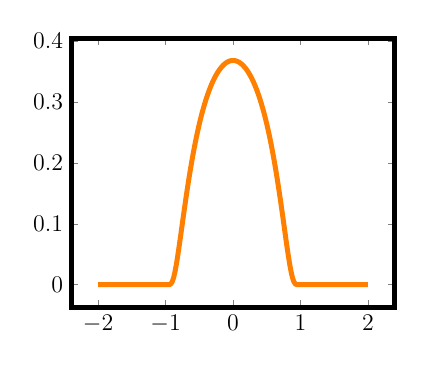
\begin{tikzpicture}[ scale=0.6,
 declare function={
    func(\x)= (\x < 1) * (0)   +
              and(\x >= -1,\x <= 1) * (exp(1/( \x*\x-1)))     +
              (\x > 1) * (0)
   ;
                  } ]

%\tikzstyle{every path}=[line width=2pt]

\begin{axis}[ ticklabel style = {font=\Large },
]
\addplot [
orange,
domain=-2:2,
samples=201,
line width=3pt
]  {func(x)};
\end{axis}
\end{tikzpicture}
\end{center}
\caption{Plot of a test function $\varphi(x)$. }
\label{2011-m-fd1}
\end{marginfigure}
}


First, note, by definition, the support  $M_\varphi=(-1,1)$,
because $\varphi (x)$   vanishes outside  $(-1,1)$).

Second, consider the differentiability of $\varphi (x)$;
that is $\varphi\in C^\infty({\Bbb R})$?
Note that
$\varphi^{(0)}=\varphi$ is continuous;
and that $\varphi^{(n)}$ is of the form
$$
   \varphi^{(n)}(x)=\left\{\begin{array}{cl}
                         {P_n(x)\over(x^2-1)^{2n}}    e^{1\over x^2-1}&\mbox{for $|x|<1$}\\
                         0&\mbox{for $|x|\geq1$,}
                    \end{array}\right.
$$
where $P_n(x)$ is a finite polynomial in $x$
 ($\varphi(u)=e^u\Longrightarrow
\varphi'(u)={d\varphi\over du}{du\over dx^2}{dx^2\over dx}=\varphi(u)
\left(-{1\over(x^2-1)^2}\right)2x$ etc.) and $[x=1-\varepsilon]\Longrightarrow
x^2=1-2\varepsilon+\varepsilon^2\Longrightarrow x^2-1=
\varepsilon(\varepsilon-2)$
\begin{eqnarray*}
   \lim_{x\uparrow1}\varphi^{(n)}(x)&=&\lim_{\varepsilon\downarrow0}
      {P_n(1-\varepsilon)\over\varepsilon^{2n}(\varepsilon-2)^{2n}}
      e^{1\over\varepsilon(\varepsilon-2)}=\\
   &=&\lim_{\varepsilon\downarrow0}{P_n(1)\over\varepsilon^{2n}2^{2n}}
      e^{-{1\over2\varepsilon}}=\left[\varepsilon={1\over R}\right]=
      \lim_{R\to\infty}{P_n(1)\over2^{2n}}R^{2n}e^{-{R\over2}}=0,
\end{eqnarray*}
because the power $e^{-x}$ of $e$
decreases stronger
than any polynomial  $x^n$.

Note that the complex continuation
$\varphi (z)$ is not an analytic function and cannot be expanded as a Taylor series on the
entire complex plane ${\Bbb C}$ although it is infinitely often
differentiable on the real axis; that is, although
$\varphi\in C^\infty({\Bbb R})$.
This can be seen from a uniqueness theorem of complex analysis.
%(z.\,B.\ Weinm\"uller-Skriptum, Seite 291):\medskip\\
Let
 $B\subseteq{\Bbb C}$ be a domain, and
let
$z_0\in B$ the limit of a sequence
$\{z_n\}\in B$, $z_n\ne z_0$.
Then it can be shown that, if two
analytic functions
$f$ and $g$ on $B$  coincide in the points $z_n$,
then they coincide on the entire domain $B$.

Now, take  $B={\Bbb R}$ and
the  vanishing analytic function $f$; that is,
$f(x)=0$.
$f(x)$ coincides with $\varphi (x)$ only in
 ${\Bbb R} - M_\varphi$.
As a result, $\varphi$ cannot be analytic.

Indeed, suppose one does not consider  the piecewise definition~(\ref{2018-m-ch-di-tf1}) of $\varphi_{\sigma, a}(x)$
(which ``gets rid'' of the ``pathologies'')
but just concentrates on its ``exponential part'' as a standalone function on the entire real continuum,
then $\exp \left\{ -\left[ 1 - \left( \frac{x-a}{\sigma }\right)^2 \right]^{-1} \right\}$ diverges at $x=a\pm\sigma$  when
computed from the ``outer regions''  $\left\vert  (x-a)/ \sigma \right\vert \ge 1$.
Therefore this function cannot be Taylor expanded around these two singular points;
and hence smoothness (that is, being in  $C^\infty$)
not necessarily implies that its continuation into the complex plain results in an analytic function. (The converse is true though: analyticity implies smoothness.)
\eproof
}

\subsection{Test function class II}

Other ``good'' test functions are \cite{schwartz}
\begin{equation}
\left\{\phi_{c,d}(x)\right\}^\frac{1}{n}
\end{equation}
obtained by choosing $n\in {\Bbb N} - 0$
and $-\infty \le c<d\le \infty$ and by defining
\begin{equation}
\phi_{c,d}(x)
=
\begin{cases}
e^{-\left( \frac{1}{x-c} + \frac{1}{d-x} \right)} & \textrm{ for }  c<x<d ,   \\
                                                0 & \textrm{ else.}
\end{cases}
\end{equation}



\subsection{Test function class III: Tempered distributions and Fourier transforms}

A particular class of ``good'' test functions -- having the property that they vanish
``sufficiently fast'' for large arguments, but are nonzero at any finite argument --
are capable of rendering Fourier transforms of generalized functions. Such generalized functions are called
{\em tempered distributions}.
\index{tempered distributions}

One example of a test function yielding tempered distribution is the {\em Gaussian function}
\index{Gaussian function}
\begin{equation}
\varphi (x)= e^{-\pi x^2}.
\label{2012-m-ch-di-td}
\end{equation}
We can multiply the Gaussian function with polynomials (or take its derivatives) and thereby obtain a particular class of test functions
inducing tempered distributions.


The Gaussian function is normalized such that
\begin{equation}
\begin{split}
\int_{-\infty}^{ \infty} \varphi (x)dx =
\int_{-\infty}^{ \infty} e^{-\pi x^2}dx \\
\qquad [\textrm{variable substitution }\; x = \frac{t}{\sqrt{\pi}}, \, dx = \frac{dt}{\sqrt{\pi}} ]\\
\qquad
= \int_{-\infty}^{ \infty}  e^{-\pi \left(\frac{t}{\sqrt{\pi}}\right)^2}d\left(\frac{t}{\sqrt{\pi}}\right)  \\
\qquad
=\frac{1}{ \sqrt{\pi} } \int_{-\infty}^{ \infty}  e^{- t^2}dt  \\
\qquad
=\frac{1}{\sqrt{\pi} } \sqrt{\pi} = 1.
\end{split}
\end{equation}
In this evaluation, we have used the {\em Gaussian integral}
\index{Gaussian integral}
\begin{equation}
I= \int_{-\infty}^{ \infty}  e^{-x^2}dx=   \sqrt{\pi},
\label{2018-m-ch-di-gi}
\end{equation}
which can be obtained by considering its square and transforming into polar coordinates $r,\theta$; that  is,
\begin{equation}
\begin{split}
I^2 =
\left(\int_{-\infty}^{ \infty}  e^{-x^2}dx\right)\left(\int_{-\infty}^{ \infty}  e^{-y^2}dy\right)  \\
\qquad =
 \int_{-\infty}^{ \infty} \int_{-\infty}^{ \infty}   e^{-\left(x^2+y^2\right)}dx \,dy   \\
\qquad =
 \int_{0}^{2\pi } \int_{0}^{ \infty}   e^{-r^2}r \, d\theta \,dr   \\
\qquad =
 \int_{0}^{2\pi }  d\theta \int_{0}^{ \infty}   e^{-r^2}r  \,dr   \\
\qquad =
 2\pi   \int_{0}^{ \infty}   e^{-r^2}r  \,dr   \\
\qquad
\left[
u=r^2, \frac{du}{dr} =2r, dr =  \frac{du}{2r}
\right]   \\
\qquad =
  \pi   \int_{0}^{ \infty}   e^{-u}  \,du  \\
\qquad =
  \pi     \left( \left. - e^{-u} \right|_{0}^{ \infty} \right)  \\
\qquad =
  \pi     \left( - e^{-\infty} + e^{0} \right)  \\
\qquad =
  \pi .
\end{split}
\label{2012-m-ch-di-gi2}
\end{equation}

The  Gaussian  test function (\ref{2012-m-ch-di-td})
has the advantage that, as has been shown in
(\ref{2012-m-ch-fa-gift}),
with a certain kind of definition for the Fourier transform,
namely  $A=2\pi $ and $B=1$  in Eq. (\ref{2011-m-efta1mg}),
its functional form does not change under Fourier transforms.
More explicitly, as derived in Eqs.
(\ref{2012-m-ch-fa-gift})
and
(\ref{2012-m-ch-fa-giftinverse}),
\begin{equation}
    {\cal F}[\varphi (x)](k)=\widetilde{\varphi} (k) =  \int_{-\infty}^\infty
                e^{-\pi  x^2}  e^{- 2\pi ikx} dx
 = e^{-{\pi k^2}} .
\end{equation}

Just as for differentiation discussed later it is possible to ``shift'' or ``transfer'' the
Fourier transformation from the distribution to the test function
as follows.
\index{Fourier transformation}
Suppose we are interested in the Fourier transform ${\cal F}[F]$ of some distribution $F$.
Then, with the convention
 $A=2\pi $ and $B=1$  adopted in Eq. (\ref{2011-m-efta1mg}), we must consider
\begin{equation}
\begin{split}
\langle  {\cal F}[F ], \varphi \rangle \equiv {\cal F}[F ][\varphi ]
=
\int_{-\infty}^\infty {\cal F}[F](x) \varphi (x) dx
\\ \qquad =
\int_{-\infty}^\infty \left[ \int_{-\infty}^\infty F(y) e^{- 2\pi ixy} dy \right] \varphi (x) dx
\\ \qquad =
\int_{-\infty}^\infty  F(y)  \left[ \int_{-\infty}^\infty \varphi (x) e^{- 2\pi ixy}  dx \right] dy
\\ \qquad =
\int_{-\infty}^\infty  F(y)  {\cal F}[ \varphi ](y) dy
\\ \qquad =
\langle  F , {\cal F}[\varphi ]\rangle \equiv F [{\cal F}[\varphi ]]
.
\end{split}
\end{equation}
in the same way we obtain the
{\em Fourier inversion}
\index{Fourier inversion}
for distributions
\begin{equation}
\langle   {\cal F}^{-1}[{\cal F}[F ]], \varphi \rangle
=
\langle   {\cal F}[{\cal F}^{-1}[F ]], \varphi \rangle
=
\langle    F  , \varphi \rangle
.
\end{equation}

Note that, in the case of test functions with compact support -- say, $\widehat{\varphi} (x) = 0$ for $\vert x \vert > a > 0$ and finite $a$
--  if the order of integrations is exchanged, the ``new test function''
\begin{equation}
{\cal F}[ \widehat{\varphi}] (y)=
\int_{-\infty}^\infty  \widehat{\varphi} (x) e^{- 2\pi ixy}  dx
=
\int_{-a}^a  \widehat{\varphi} (x) e^{- 2\pi ixy}  dx
\end{equation}
obtained through a Fourier transform of  $\widehat{\varphi} (x)$,
does not necessarily inherit a compact support  from $\widehat{\varphi} (x)$;
in particular,
${\cal F}[ \widehat{\varphi}] (y)$
may not necessarily vanish [i.e.  ${\cal F}[ \widehat{\varphi}] (y) = 0$] for $\vert y \vert > a > 0$.


{
\color{blue}
\bexample
Let us, with these conventions, compute the Fourier transform of the tempered Dirac delta distribution.
Note that, by the very definition of the  Dirac delta distribution,
\begin{equation}
\begin{split}
\langle    {\cal F}[\delta  ] , \varphi \rangle
=
\langle   \delta , {\cal F}[\varphi ]\rangle
\\ =
{\cal F}[\varphi](0)=  \int_{-\infty}^\infty  e^{- 2\pi ix 0} \varphi (x) dx
=  \int_{-\infty}^\infty  1 \varphi (x) dx
=  \langle   1 , \varphi \rangle
.
\end{split}
\end{equation}
Thus we may identify  ${\cal F}[\delta  ]$ with $1$; that is,
\begin{equation}
{\cal F}[\delta  ] = 1
.
\end{equation}
This is an extreme example of an {\em infinitely concentrated} object whose Fourier transform is
{\em infinitely spread out}.

A very similar calculation renders the tempered distribution associated with the Fourier transform of the shifted Dirac delta distribution
\begin{equation}
{\cal F}[\delta_y  ] = e^{- 2\pi ix y}
.
\end{equation}
\eexample
}

Alas, we shall pursue a different, more conventional, approach, sketched in Section \ref{2012-m-ch-di-ftgeneraldefcon}.

\subsection{Test function class $C^\infty$}

If the generalized functions are ``sufficiently concentrated'' so that they themselves guarantee that the terms
$g(\infty)\varphi(\infty)$ as well as $g(-\infty)\varphi(-\infty)$
in Eq. (\ref{2012-m-ch-di-desiderata}) to vanish,
we may just require the test functions to be infinitely differentiable -- and thus in $C^\infty$ --
for the sake of making possible a transfer of differentiation.
(Indeed, if we are willing to sacrifice even infinite differentiability, we can widen this class of test functions even more.)
We may, for instance, employ constant functions such as $\varphi (x)=1$ as test functions,
thus giving meaning to, for instance,
$\langle \delta , 1\rangle= \int_{-\infty}^\infty \delta (x) dx$,
or
$\langle f(x)\delta , 1\rangle= \langle f(0)\delta , 1\rangle= f(0)\int_{-\infty}^\infty  \delta (x) dx$.

However, one should keep in mind that constant functions, or arbitrary smooth functions, do not comply with the generally accepted notion of a test function.
Test functions are usually assumed to have either a compact support or at least decrease sufficiently fast to allow,
say,  vanishing nonintegral surface terms in integrations by parts.

\section{Derivative of distributions}

Equipped with ``good'' test functions
which have a finite support and are
infinitely often (or at least sufficiently often) differentiable,
we can now give meaning to the transferral  of differential quotients from
the objects entering the integral towards the test function by {\em partial integration}.
First note again that $(uv)' = u'v+uv'$
and thus
$\int (uv)' = \int u'v+\int uv'$
and finally   $\int u'v = \int (uv)'  -\int uv'$.
Hence,     by identifying $u$ with $g$, and $v$ with the test function $\varphi$, we obtain
\begin{equation}
\begin{split}
\langle {F}' , \varphi \rangle \equiv {F}'\left[\varphi\right] =
\int_{-\infty}^\infty
\left( \frac{d}{dx} F(x)\right) \varphi (x) dx
\\
\qquad =
\underbrace{\left. F(x) \varphi (x) \right|_{x=-\infty}^\infty}_{=0}
- \int_{-\infty}^\infty
F(x)\left( \frac{d}{dx} \varphi (x) \right) dx \\
\qquad =
- \int_{-\infty}^\infty
F(x)\left( \frac{d}{dx} \varphi (x) \right) dx \\
\qquad =-F\left[\varphi  '\right] \equiv - \langle {F} , \varphi '\rangle .
\end{split}
\end{equation}
By induction
\begin{equation}
\left\langle \frac{d^{n}}{dx^{n}}{F} , \varphi \right\rangle
\equiv
\langle {F}^{(n)} , \varphi \rangle \equiv F^{(n)}\left[\varphi\right]
 = (-1)^n F\left[\varphi  ^{(n)}\right]
 = (-1)^n   \langle {F} , \varphi^{(n)}\rangle.
\end{equation}



{
\color{blue}
\bexample

In anticipation of the definition (\ref{2018-m-ch-di-delta}) of the delta function by $\delta [\varphi ]=\varphi (0)$
we immediately obtain its derivative by $\delta' [\varphi ]= - \delta[\varphi '  ]=-\varphi' (0)$.


For the sake of a further example using   adjoint identities
\index{adjoint identities},
to swapping products and differentiations forth and back
through the $F$--$\varphi$ pairing, let us compute
$g(x)\delta' (x)$ where $g \in C^\infty$; that is
\begin{equation}
\begin{split}
g \delta' [\varphi ] \equiv
\langle g \delta'   , \varphi \rangle
=
\langle \delta'   , g  \varphi \rangle
 =
- \langle \delta   , (g  \varphi )'\rangle
 =  \\
- \langle \delta   ,  g  \varphi  '+ g'  \varphi  \rangle
 =
-  g(0)  \varphi ' (0) - g'(0)  \varphi(0)
 =
  \langle g(0) \delta '   -  g'(0)\delta , \varphi   \rangle
\\ \equiv
\left(g(0)\delta ' -g'(0)\delta \right) [\varphi ]
= g(0)\delta '[\varphi] -g'(0)\delta [\varphi ]
.
\end{split}
\end{equation}
\eexample
}
Therefore,  in the functional sense,
\begin{equation}
g(x)\delta' (x)=g(0) \delta '(x)   -  g'(0)\delta (x) .
\label{2012-m-ch-di-sederi}
\end{equation}




\section{Fourier transform  of distributions}
\label{2012-m-ch-di-ftgeneraldefcon}

We mention without proof that, if $\{ f_n(x)\}$ is a sequence of functions converging, for $n\rightarrow \infty$,
toward a function $f$ in the functional sense (i.e. {\it via}
integration of $f_n$ and $f$ with ``good'' test functions),
then the Fourier transform $\widetilde f$ of $f$ can be defined by \cite{Lighthill,Howell,doi:10.1080/0020739900210418}
\begin{equation}
\begin{split}
 {\cal F}[f]=\widetilde{f}(k)= \lim_{n\rightarrow \infty}
 \int_{-\infty}^\infty  f_n(x) e^{-i{kx}} dx
.
\end{split}
\end{equation}

While this represents a method to calculate  Fourier transforms of distributions, there are other, more direct ways of
obtaining them.
These were mentioned earlier.




\section{Dirac  delta function}
\index{Dirac delta function}
\index{delta function}



The theory of distributions has been stimulated by physics.
Historically, the Heaviside step function, which will be discussed later --
was used for the description of electrostatic pulses.

In the days when Dirac developed quantum mechanics
(cf. \S 15 of Ref.~ \cite[-10mm]{dirac})
there was a need to define
``singular scalar products'' such as ``$\langle x \mid y \rangle = \delta (x-y)$,''
with some generalization of the Kronecker delta function $\delta_{ij}$, depicted in Fig.~\ref{2011-m-fdeltaplot},
which is zero whenever $x\neq y$;
and yet at the same time ``large enough'' and
``needle shaped'' as depicted in Fig.~\ref{2011-m-fdeltaplot} to yield unity when
integrated over the entire reals; that is, ``$\int_{-\infty}^\infty \langle x \mid y \rangle dy =\int_{-\infty}^\infty \delta (x-y) dy =1$.''
\begin{marginfigure}%
\begin{center}
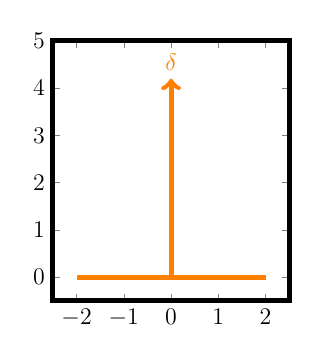
\begin{tikzpicture}[ scale=0.6,
 declare function={
    func(\x)= 0;
                  } ]

\begin{axis}[
ticklabel style = {font=\Large },
ymin=-0.5,
ymax=5.0,
xmin=-2.5,
xmax=2.5,
height=5.5cm,width=5cm,
scale only axis
]
\addplot [
orange,
domain=-2:2,
%samples=201,
line width=3pt
]  {func(x)};

\draw[orange,line width=3pt,->] (axis cs:0,0) --   (axis cs:0,4.2) node[above]{{\Large $\delta$}};

\end{axis}
\end{tikzpicture}
\end{center}
\caption{Dirac's $\delta$-function as a ``needle shaped'' generalized function.}
  \label{2011-m-fdeltaplot}
\end{marginfigure}


Naturally, such ``needle shaped functions'' were viewed suspiciously by many mathematicians
at first, but later they embraced these types of functions
\cite[0mm]{gelfand:1964:gf} by developing a theory of
{\em functional analysis}
\index{functional analysis},
{\em generalized functions}
\index{generalized functions}
or, by another naming,
{\em distributions}.
\index{distributions}

In what follows we shall first define the Dirac delta function by delta sequences; that is, by sequences of functions which render the
delta function in the limit.
Then the delta function will be formally defined in~(\ref{2018-m-ch-di-delta}) by $\delta [\varphi ]=\varphi (0)$.

\subsection{Delta sequence}
One of the first attempts to formalize these objects with ``large discontinuities''
was in terms
of functional limits.
Take, for instance, the {\em delta sequence}
\index{delta sequence}
of ``strongly peaked'' pulse functions
depicted in Fig.~\ref{2011-m-fdeltaplotnseq};
defined by
\begin{equation}
\delta_n(x-y) =
\left\{
\begin{array}{rl}
n & \textrm{ for } y - \frac{1}{2n}  < x < y+ \frac{1}{2n} \\
0& \textrm{ else. }
\end{array}
\right.
\label{2011-m-deltseq}
\end{equation}
In  the functional sense the ``large $n$ limit''   of
the sequences $\{f_n(x-y)\}$
 becomes the delta function $\delta (x-y)$:
\begin{equation}
\lim_{n\rightarrow \infty} \delta_n(x-y)= \delta (x-y) ;
\end{equation}
that is,
\begin{equation}
\lim_{n\rightarrow \infty} \int \delta_n(x-y) \varphi (x) dx = \delta_y [\varphi ]=\varphi (y).
\end{equation}

Note that, for all $n\in \mathbb{N}$ the area of $\delta_n(x-y)$ above the $x$-axes
is $1$ and independent of $n$, since the width is $1/n$ and the height is $n$, and the of width and height is $1$.
\begin{marginfigure}%
\begin{center}
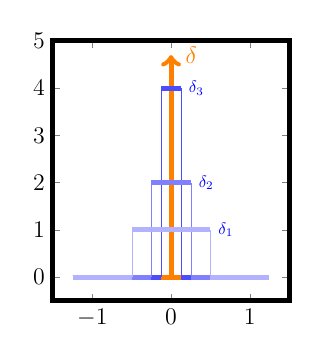
\begin{tikzpicture}[ scale=0.6,
 declare function={
    func(\x)= 0;
    func1(\x)= (\x <= 1/2) * (0)   +
              and(\x >= -1/2,\x <= 1/2) * (1)     +
              (\x >= 1/2) * (0) ;
    func2(\x)= (\x < 1/4) * (0)   +
              and(\x >= -1/4,\x <= 1/4) * (2)     +
              (\x > 1/4) * (0) ;
    func3(\x)= (\x < 1/8) * (0)   +
              and(\x >= -1/8,\x <= 1/8) * (4)     +
              (\x > 1/8) * (0) ;
                  } ]

\begin{axis}[
ticklabel style = {font=\Large },
ymin=-0.5,
ymax=5.0,
xmin=-1.5,
xmax=1.5,
height=5.5cm,width=5cm,
scale only axis
]

\addplot [
orange,
domain=-1.25:1.25,
%samples=201,
line width=3pt
]  {func(x)};

\draw[orange,line width=3pt,->] (axis cs:0,0) -- (axis cs:0,4.7) node[right]{{\Large $\;\delta$}};

\addplot [
blue!70,
domain=-1/8:1/8,
% samples=301,
line width=3pt
]  {func3(x)} node[right]{{\color{blue}$\delta_3$}};

\draw[blue!70,line width=0.2pt] (axis cs:-1/8,0) -- (axis cs:-1/8,4);
\draw[blue!70,line width=0.2pt] (axis cs:1/8,0) -- (axis cs:1/8,4);

\draw[blue!70,line width=3pt] (axis cs:-1.25,0) -- (axis cs:-1/8,0);
\draw[blue!70,line width=3pt] (axis cs:1/8,0) -- (axis cs:1.25,0);

\addplot [
blue!50,
domain=-0.25:0.25,
% samples=301,
line width=3pt
]  {func2(x)} node[right]{{\color{blue}$\delta_2$}};

\draw[blue!50,line width=0.2pt] (axis cs:-1/4,0) -- (axis cs:-1/4,2);
\draw[blue!50,line width=0.2pt] (axis cs:1/4,0) -- (axis cs:1/4,2);

\draw[blue!50,line width=3pt] (axis cs:-1.25,0) -- (axis cs:-1/4,0);
\draw[blue!50,line width=3pt] (axis cs:1/4,0) -- (axis cs:1.25,0);

\addplot [
blue!30,
domain=-0.5:0.5,
% samples=301,
line width=3pt
]  {func1(x)} node[right]{{\color{blue}$\delta_1$}};

\draw[blue!30,line width=0.2pt] (axis cs:-0.5,0) -- (axis cs:-0.5,1);
\draw[blue!30,line width=0.2pt] (axis cs:0.5,0) -- (axis cs:0.5,1);

\draw[blue!30,line width=3pt] (axis cs:-1.25,0) -- (axis cs:-0.5,0);
\draw[blue!30,line width=3pt] (axis cs:0.5,0) -- (axis cs:1.25,0);


\end{axis}
\end{tikzpicture}
\end{center}
\caption{Delta sequence approximating Dirac's $\delta$-function as a more and more ``needle shaped'' generalized function.}
  \label{2011-m-fdeltaplotnseq}
\end{marginfigure}


{
\color{blue}
\bexample
Let us proof that the sequence $\{ \delta_n\}$ with
$$\delta_n(x-y) =
\left\{
\begin{array}{rl}
n & \textrm{ for } y - \frac{1}{2n}  < x < y+ \frac{1}{2n} \\
0& \textrm{ else }
\end{array}
\right.$$
defined in Eq. (\ref{2011-m-deltseq}) and depicted
in Fig.
\ref{2011-m-fdeltaplotnseq}
is a delta sequence;
that is, if, for large $n$, it converges to $\delta$ in a functional sense.
In order to verify this claim, we have to integrate $\delta_n(x)$
with ``good'' test functions $ \varphi (x)$ and take the limit $n\rightarrow \infty$;
if the result is $ \varphi (0)$, then we can identify $\delta_n(x)$ in this limit with $\delta (x)$
(in the functional sense).
Since $\delta_n(x)$ is uniform convergent, we can exchange the limit with the integration; thus
\begin{equation}
\begin{split}
\lim_{n\rightarrow \infty} \int_{-\infty}^\infty \delta_n(x-y) \varphi (x) dx \\
 \textrm{[variable transformation:}  \\
  x'=x-y, x= x'+y, dx' =  dx, -\infty\le x' \le \infty \textrm{]} \\
 =
\lim_{n\rightarrow \infty} \int_{-\infty}^\infty \delta_n(x') \varphi (x'+y) dx'
 =
\lim_{n\rightarrow \infty} \int_{- \frac{1}{2n}}^\frac{1}{2n} n \varphi (x'+y) dx'    \\
 \textrm{[variable transformation:}  \\
  u=2nx', x'=\frac{u}{2n},
   du = 2n dx', -1\le u \le 1\textrm{]} \\
 = \lim_{n\rightarrow \infty} \int_{- 1}^1 n \varphi (\frac{ u}{2n}+y) \frac{du}{2n}
 =
\lim_{n\rightarrow \infty} \frac{1}{2} \int_{- 1}^1 \varphi (\frac{ u}{2n}+y) du     \\
 =
\frac{1}{2} \int_{- 1}^1 \lim_{n\rightarrow \infty} \varphi (\frac{ u}{2n}+y) du
  =
\frac{1}{2} \varphi (y) \int_{- 1}^1  du
  =
\varphi (y)
.
\end{split}
\end{equation}
Hence, in the functional sense,
this limit yields the shifted $\delta$-function $\delta_y$.
Thus we obtain
$
\lim_{n\rightarrow \infty} \delta_n[\varphi] = \delta_y [\varphi] = \varphi (y)
$.
\eexample
}


Other delta sequences can be {\it ad hoc}  enumerated as follows.
They all converge towards the delta function in the sense of linear functionals (i.e. when integrated over a test function).
\begin{eqnarray}
\delta_n(x)
&=& \frac{n}{\sqrt{\pi}} e^{-n^2 x^2},
\label{2012-m-ch-di-g1}\\
&=&
\frac{1}{\pi}\frac{n}{1+ n^2x^2},    \label{2012-m-ch-di-l1} \\
&=&
\frac{1}{\pi}   \frac{\sin (n x)}{ x}, \label{2012-m-ch-di-d1}\\
&=&
= (1\mp i)\left( {n\over 2\pi }\right)^{1\over 2} e^{\pm inx^2}  \\
&=&
\frac{1}{\pi x}  \frac{e^{inx}-e^{-inx}}{2i} ,\\
&=&
\frac{1}{\pi}  \frac{n  e^{-x^2}}{1+n^2x^2} ,\\
&=&
\frac{1}{2\pi } \int_{-n}^n e^{ixt} dt  = \frac{1}{2\pi i x} \left. e^{ixt}\right|_{-n}^n    ,\\
&=&
\frac{1}{2\pi} \frac{\sin \left[\left( n+\frac{1}{2}\right) x \right]  }{\sin \left( \frac{1}{2}x \right)   },\\
&=&
\frac{n}{ \pi}\left(\frac{\sin (nx)}{nx}\right)^2.
\end{eqnarray}
Other commonly used limit forms of the $\delta $-function are the Gaussian, Lorentzian, and Dirichlet forms
\begin{eqnarray}
\delta_\epsilon (x) &=&   \frac{1}{\sqrt{\pi } \epsilon } e^{-\frac{x^2}{\epsilon^2}} ,
\label{2012-m-ch-di-g2} \\
&=&  \frac{1}{\pi} \frac{\epsilon }{x^2+\epsilon^2}
=   {1\over 2\pi i}
\left(
{1 \over x-i\epsilon }
-
{1 \over x+i\epsilon }
 \right)
 , \label{2012-m-ch-di-l2}  \\
&=&  \frac{1}{\pi } \frac{\sin \left(\frac{x}{\epsilon }\right)}{x} ,  \label{2012-m-ch-di-d2}
\end{eqnarray}
respectively.
Note that
(\ref{2012-m-ch-di-g2}) corresponds to (\ref{2012-m-ch-di-g1}),
(\ref{2012-m-ch-di-l2}) corresponds to (\ref{2012-m-ch-di-l1}) with $\epsilon=n^{-1}$,
and
(\ref{2012-m-ch-di-d2}) corresponds to (\ref{2012-m-ch-di-d1}).
Again, the limit
$
\delta (x)= \lim_{\epsilon \rightarrow 0} \delta_\epsilon (x)
$
has to be understood in the functional sense; that is, by integration over a test function,
so that
\begin{equation}
\lim_{\epsilon \rightarrow 0} \delta_\epsilon [\varphi]=
\int \delta_\epsilon (x) \varphi (x) dx  =    \delta [\varphi]=\varphi (0).
\end{equation}





\subsection{$\delta \left[ \varphi \right]$ distribution}
\index{delta function}

The distribution (linear functional) associated with the $\delta$ function
can be defined by mapping any test function into a scalar as follows:
\begin{equation}
\delta_y [\varphi ]\stackrel{{\tiny \textrm{ def }}}{=}\varphi (y);
\label{2018-m-ch-di-delta}
\end{equation}
or, as it is often expressed,
\begin{equation}
\int_{-\infty}^\infty
\delta(x-y) \varphi (x) dx = \varphi(y).
\end{equation}
Other common ways of expressing this {\em delta function distribution} is by writing
\begin{equation}
\delta(x-y) \longleftrightarrow
\langle \delta_y , \varphi \rangle \equiv
\langle \delta_y \vert \varphi \rangle \equiv
\delta_y [\varphi] = \varphi (y).
\end{equation}
For $y=0$, we just obtain
\begin{equation}
\delta(x) \longleftrightarrow
\langle \delta , \varphi \rangle \equiv
\langle \delta \vert \varphi \rangle \equiv
\delta [\varphi] \stackrel{{\tiny \textrm{ def }}}{=} \delta_0 [\varphi] =  \varphi (0).
\end{equation}
Note that $\delta_y[\varphi]$ is a singular distribution,
as no regular function is capable of such a performance.
\index{singular distribution}



\subsection{Useful formul\ae{} involving $\delta$}

The following formul\ae{} are sometimes enumerated without proofs.


 \begin{equation}
 f (x)\delta (x-x_0)
 =
f (x_0)\delta (x-x_0)
\label{2018-m-ch-di-totenk}
 \end{equation}
{\color{OliveGreen}
\bproof
This results from a direct application of Eq.~(\ref{2013-m-ch-di-multipl}); that is,
 \begin{equation}
f(x) \delta
[\varphi ]
=
\delta
\left[  f  \varphi \right]
=
f(0)\varphi(0) = f(0)   \delta
[\varphi ]
,
 \end{equation}
and
 \begin{equation}
f(x) \delta_{x_0}
[\varphi ]
=
\delta_{x_0}
\left[  f  \varphi \right]
=
f({x_0})\varphi({x_0}) = f({x_0})   \delta_{x_0}
[\varphi ]
.
 \end{equation}
For a more explicit direct proof, note that formally
 \begin{equation}
 \begin{split}
\int _{-\infty}^\infty f (x)\delta (x-x_0)  \varphi(x) dx
=
\int _{-\infty}^\infty\delta (x-x_0)  ( f (x)\varphi(x) ) dx = f(x_0) \varphi(x_0)
,
 \end{split}
 \end{equation}
and hence $f(x) \delta_{x_0}[ \varphi ] =   f(x_0)\delta_{x_0}[ \varphi ]$.
\eproof
}


 \begin{equation}
 \delta (-x)=\delta (x)
 \end{equation}
% S. Gro\ss mann, {\sl Funktionalanalysis I} (Akademische Verlagsgesellschaft, Wiesbaden 1975)
{\color{OliveGreen}
\bproof
For a proof, note that $\varphi (x)\delta (-x) = \varphi (0)\delta (-x)$, and that, in particular,
with the substitution $x \rightarrow -x$ and a redefined test function $\psi (x) =\varphi(-x)$:
 \begin{equation}
 \begin{split}
\int _{-\infty}^\infty \delta (-x)  \varphi(x) dx   =
 \int_\infty ^{-\infty}\delta (-(-x)) \underbrace{\varphi(-x)}_{=\psi(x)} d(-x) \\
   =
-\underbrace{\psi(0)}_{\varphi(0)} \int _\infty ^{-\infty}\delta (x)  d x     =
\varphi(0) \int _{-\infty}^\infty \delta (x)  d x =\varphi(0)=\delta[\varphi].
 \end{split}
 \end{equation}
\eproof
}


For the $\delta$ distribution with its ``extreme concentration'' at the origin, a ``nonconcentrated test function'' suffices; in particular, a constant ``test'' function
-- even without compact support and sufficiently strong damping at infinity --
such as $\varphi (x) = 1$ is fine.
This is the reason why test functions need not show up explicitly in expressions, and, in particular, integrals, containing $\delta$.
Because, say, for suitable functions $g(x)$ ``well behaved'' at the origin, formally by invoking~(\ref{2018-m-ch-di-totenk})
 \begin{equation}
 \begin{split}
\int_{-\infty}^{\infty} g(x)\delta(x-y) \,dx =
\int_{-\infty}^{\infty} g(y)\delta(x-y) \,dx \\=
g(y)\int_{-\infty}^{\infty} \delta(x-y)  \,dx =g(y).
 \end{split}
\end{equation}

% S. Gro\ss mann, {\sl Funktionalanalysis I} (Akademische Verlagsgesellschaft, Wiesbaden 1975)
 \begin{equation}
 x\delta (x)=0
 \end{equation}
 % S. Gro\ss mann, {\sl Funktionalanalysis I} (Akademische Verlagsgesellschaft, Wiesbaden 1975)
{\color{OliveGreen}
\bproof
For a proof invoke~(\ref{2018-m-ch-di-totenk}), or explicitly consider
 \begin{equation}
x \delta
[\varphi ]
=
\delta
\left[  x  \varphi \right]
=
0\varphi(0) = 0.
 \end{equation}
\eproof
}
For $a\neq 0$,
 \begin{equation}
 \delta (ax)={1\over \vert a\vert }\delta (x),
\label{2011-m-distdp}
 \end{equation}
and, more generally,
 \begin{equation}
 \delta (a(x-x_0))={1\over \vert a\vert }\delta (x-x_0)
\label{2011-m-distdpmg}
 \end{equation}
 % S. Gro\ss mann, {\sl Funktionalanalysis I} (Akademische Verlagsgesellschaft, Wiesbaden 1975)
{\color{OliveGreen}
\bproof
For the sake of a proof,  consider the case $a>0$ as well as $x_0=0$ first:
 \begin{equation}
 \begin{split}
\int _{-\infty}^\infty \delta (ax)  \varphi (x)  dx
\\
  [\textrm{variable substitution }\; y = ax, x=\frac{y}{a}, dx=\frac{1}{a} dy]\\
  =
\frac{1}{a}\int _{-\infty}^\infty \delta (y)  \varphi\left (\frac{y}{a}\right) dy  \\
  =    \frac{1}{a}  \varphi (0)=    \frac{1}{\vert a\vert}  \varphi (0);
 \end{split}
 \end{equation}
and, second, the case $a<0$:
 \begin{equation}
 \begin{split}
\int _{-\infty}^\infty \delta (ax)  \varphi (x)  dx     \\
\qquad [\textrm{variable substitution }\; y = ax, x=\frac{y}{a}, dx=\frac{1}{a} dy]\\
\qquad =
\frac{1}{a}\int _\infty^{-\infty} \delta (y)  \varphi\left (\frac{y}{a}\right) dy \\
\qquad =
- \frac{1}{a}\int _{-\infty}^\infty \delta (y)  \varphi\left (\frac{y}{a}\right) dy       \\
\qquad =   - \frac{1}{a}  \varphi (0)=    \frac{1}{\vert a\vert}  \varphi (0).
 \end{split}
 \end{equation}
In the case of $x_0\neq 0$ and $\pm a>0$, we obtain
\begin{equation}
 \begin{split}
\int _{-\infty}^\infty \delta (a(x-x_0))  \varphi (x)  dx
\\
 [\textrm{variable substitution }\; y = a(x-x_0), x=\frac{y}{a}+x_0, dx=\frac{1}{a} dy]\\
 =
\pm \frac{1}{a}\int _{-\infty}^\infty \delta (y)  \varphi \left(\frac{y}{a}+x_0\right) dy  \\
 =    \pm \frac{1}{a}  \varphi (0)=\frac{1}{|a|}  \varphi (x_0).
 \end{split}
 \end{equation}
\eproof
}

If there exists a simple singularity $x_0$ of $f(x)$ in the
integration interval, then
\begin{equation}
 \delta (f(x))={1\over \vert f'(x_0)\vert }\delta(x-x_0)
.
 \end{equation}
% S. Gro\ss mann, {\sl Funktionalanalysis I} (Akademische Verlagsgesellschaft, Wiesbaden 1975)
More generally,  if $f$ has only simple roots and $f'$ is nonzero there,
\begin{equation}
 \delta (f(x))=\sum_{x_i}{\delta(x-x_i)\over \vert f'(x_i)\vert }
\label{2011-m-distdp1}
 \end{equation}
where the sum extends over all simple roots $x_i$ in
the integration interval.
In particular,
 \begin{equation}
 \delta (x^2-x_0^2)={1\over 2\vert x_0\vert }[\delta (x-x_0)+\delta
 (x+x_0)] \end{equation}
% S. Gro\ss mann, {\sl Funktionalanalysis I} (Akademische Verlagsgesellschaft, Wiesbaden 1975)
{\color{OliveGreen}
\bproof
For a sloppy proof, note that, since $f$ has only simple roots
\marginnote{An example is  a polynomial of degree $k$ of the form
$f= A \prod_{i=1}^k (x-x_i)$;
with mutually distinct $x_i$, $1\le i \le k$.},
it can be expanded around these roots by
\index{order of}
\marginnote{The symbol ``$O$'' stands for ``of the order of'' or ``absolutely bound by'' in the following way:
if $g(x)$ is a positive function,  then $f(x)=O(g(x))$ implies that there exist a positive real number $m$
such that $\vert f(x) \vert < m g(x)$. \label{2018-mm-ch-di-otof}}
\[
\begin{split}
f(x) =\underbrace{f(x_0)}_{=0} +(x-x_0) f'(x_0) + O\left((x-x_0)^2\right) \\
= (x-x_0) \left[ f'(x_0) +  O\left(\vert x-x_0 \vert \right) \right] \approx  (x-x_0) f'(x_0)
\end{split}
\]
with nonzero $f'(x_0) \in {\Bbb R}$.
\marginnote{The simplest nontrivial case is $f(x) = a + bx  = b \left(\frac{a}{b}+x\right)$,
for which $x_0 = -\frac{a}{b}$ and $f' \left(x_0=\frac{a}{b}\right) = b$.}
By identifying  $f'(x_0)$ with $a$ in
Eq. (\ref{2011-m-distdp})
we obtain
Eq. (\ref{2011-m-distdp1}).

For a proof~\cite{Cortizo-95} the integration which originally extend over the set of real numbers $\mathbb{R}$
can be reduced to intervals $[x_i-r_i,x_i+r_i]$, containing the roots $x_i$ of $f(x)$.
so that  the ``radii'' $r_i$  are ``small enough'' for these intervals to be pairwise disjoint,
and $f(x) \neq 0$ for any $x$ outside of the union set of these intervals.
Therefore the integration over the entire reals can be reduced to the sum of the integrations
over the intervals; that is,
\begin{equation}
\int_{-\infty}^{+\infty} \delta (f(x)) \varphi(x) dx
=
\sum_i
\int_{x_i-r_i}^{x_i+r_i} \delta (f(x)) \varphi(x) dx
.
\label{2017-m-ch-di-sum}
\end{equation}
The terms in the sum can be evaluated separately; so let us concentrate on the $i$'th term
$\int_{x_i-r_i}^{x_i+r_i} \delta (f(x)) \varphi(x) dx    $ in~(\ref{2017-m-ch-di-sum}).
Restriction to a sufficiently small single region $[x_i-r_i,x_i+r_i]$, and the assumption of simple roots
guarantees that $f(x)$ is invertible within that region; with the inverse $f_i^{-1}$; that is,
\begin{equation}
f_i^{-1}(f(x))=x \text{ for } x \in  [x_i-r_i,x_i+r_i]
;
\end{equation}
and, in particular, $f(x_i)=0$ and $f_i^{-1}(0) =f_i^{-1}(f(x_i))=x_i$.
Furthermore, this inverse $f_i^{-1}$ is monotonic, differentiable and its derivative is nonzero within $[f(x_i-r_i),f(x_i+r_i)]$.
Define
\begin{equation}
\begin{split}
y = f(x),\\
x = f_i^{-1} (y), \text{ and}\\
dy = f'(x) dx , \text{ or } dx = \frac{dy}{f'(x)}
,
\end{split}
\end{equation}
 so that, for  $f'(x_i)>0$,
\begin{equation}
\begin{split}
\int_{x_i-r_i}^{x_i+r_i} \delta (f(x)) \varphi(x) dx
=
\int_{x_i-r_i}^{x_i+r_i} \delta (f(x)) \frac{\varphi(x)}{f'(x)} f'(x)  dx   \\
=
\int_{f(x_i-r_i)}^{f(x_i+r_i)} \delta (y) \frac{\varphi(f_i^{-1} (y))}{f'(f_i^{-1} (y))}   dy  \\
%=
%\int_{f(x_i-r_i)}^{f(x_i+r_i)} \delta (y) \frac{\varphi(f_i^{-1} (y))}{f'(f_i^{-1} (y))}   dy
=  \frac{\varphi(f_i^{-1} (0))}{f'(f_i^{-1} (0))}
=  \frac{\varphi(f_i^{-1} (f(x_i)))}{f'(f_i^{-1} (f(x_i)))}
=  \frac{\varphi( x_i)}{f'( x_i )}.
\end{split}
\end{equation}
Likewise, for  $f'(x_i)<0$,
\begin{equation}
\begin{split}
\int_{x_i-r_i}^{x_i+r_i} \delta (f(x)) \varphi(x) dx
=
\int_{x_i-r_i}^{x_i+r_i} \delta (f(x)) \frac{\varphi(x)}{f'(x)} f'(x)  dx   \\
=
\int_{f(x_i-r_i)}^{f(x_i+r_i)} \delta (y) \frac{\varphi(f_i^{-1} (y))}{f'(f_i^{-1} (y))}   dy
=
- \int_{f(x_i+r_i)}^{f(x_i-r_i)} \delta (y) \frac{\varphi(f_i^{-1} (y))}{f'(f_i^{-1} (y))}   dy  \\
=  - \frac{\varphi(f_i^{-1} (0))}{f'(f_i^{-1} (0))}
=  - \frac{\varphi(f_i^{-1} (f(x_i)))}{f'(f_i^{-1} (f(x_i)))}
=  - \frac{\varphi( x_i)}{f'( x_i )} .
\end{split}
\end{equation}
\eproof
}


 %\begin{equation}
 %\delta '(f(x))=
 %\sum_{i=0}^N
 %{f'' (x_i)\over \vert f'(x_i)\vert ^3}
 %\delta (x-x_i) +
 %\sum_{i=0}^N
 %{f' (x_i)\over \vert f'(x_i)\vert ^3}
 %\delta ' (x-x_i)
 %\end{equation}
% Testbeispiel Lakatha
 \begin{equation}
 \vert x\vert \delta (x^2)=\delta (x)
 \end{equation}
% S. Gro\ss mann, {\sl Funktionalanalysis I} (Akademische Verlagsgesellschaft, Wiesbaden 1975)
{\color{OliveGreen}
\bproof
For a proof consider
 \begin{equation}
 \begin{split}
\vert x \vert \delta (x^2)[\varphi ]
=
\int_{-\infty}^{\infty}\vert x \vert \delta (x^2)\varphi (x) dx\\
=
\lim_{a\rightarrow 0^+}
\int_{-\infty}^{\infty}\vert x \vert \delta (x^2-a^2)\varphi (x) dx    \\
=
\lim_{a\rightarrow 0^+}
\int_{-\infty}^{\infty}\frac{\vert x \vert}{2a} \left[ \delta (x -a ) + \delta (x + a )\right] \varphi (x) dx \\
=
\lim_{a\rightarrow 0^+} \left[
\int_{-\infty}^{\infty}\frac{\vert x \vert}{2a}   \delta (x -a ) \varphi (x) dx  +
\int_{-\infty}^{\infty}\frac{\vert x \vert}{2a}  \delta (x + a )\varphi (x) dx \right]  \\
=
\lim_{a\rightarrow 0^+} \left[
 \frac{\vert a \vert}{2a}   \varphi   (a)   +
 \frac{\vert -a \vert}{2a}  \varphi (-a)   \right]  \\
=
\lim_{a\rightarrow 0^+} \left[
 \frac{1}{2 }     \varphi (a)    +
 \frac{1}{2 }  \varphi (-a)   \right]  \\
=
\frac{1}{2 }     \varphi (0)   +
 \frac{1}{2 }  \varphi (0)
= \varphi (0)
=
\delta[\varphi ]
.
 \end{split}
 \end{equation}
\eproof
}

 \begin{equation}
 -x\delta '(x)=\delta (x),
 \end{equation}
% S. Gro\ss mann, {\sl Funktionalanalysis I} (Akademische Verlagsgesellschaft, Wiesbaden 1975)
which is a direct consequence of Eq. (\ref{2012-m-ch-di-sederi}).
{\color{OliveGreen}
\bproof
More explicitly, we can use partial integration and obtain
 \begin{equation}
 \begin{split}
-\int _{-\infty}^\infty x \delta' (x)  \varphi (x)  dx  \\
 =  - \left. x \delta (x)\right|_{-\infty}^\infty  + \int _{-\infty}^\infty \delta (x)
\frac{d}{dx}\left(x \varphi (x)\right)dx\\
 =
\int _{-\infty}^\infty \delta (x)
x \varphi' (x)  dx
+
\int _{-\infty}^\infty \delta (x)
\varphi (x) dx\\
 =
0 \varphi' (0)  +
\varphi (0)= \varphi (0).
 \end{split}
 \end{equation}
\eproof
}

 \begin{equation}
 \delta^{(n)}(-x) =(-1)^n\delta^{(n)}(x)
,
 \end{equation}
where the index $^{(n)}$ denotes $n$-fold differentiation,
can be proven by
[recall that, by the chain rule of differentiation, $\frac{d}{dx} \varphi (-x)  = - \varphi' (-x)$]
{\color{OliveGreen}
\bproof
 \begin{equation}
 \begin{split}
\int _{-\infty}^\infty \delta^{(n)} (-x)  \varphi (x)  dx  \\
[\textrm{variable substitution }\; x \rightarrow -x]\\
=
-\int _\infty^{-\infty} \delta^{(n)} (x)  \varphi (-x) dx
=
\int _{-\infty}^\infty \delta^{(n)} (x)  \varphi (-x) dx \\
 =
(-1)^n \int _{-\infty}^\infty \delta (x) \left[ \frac{d^n}{dx^n}  \varphi  (-x)\right] dx \\
 =
(-1)^n \int _{-\infty}^\infty \delta (x) \left[(-1)^n  \varphi^{(n)} (-x)\right] dx \\
 =
\int _\infty^{-\infty} \delta (x) \varphi^{(n)} (-x) dx \\
[\textrm{variable substitution }\; x \rightarrow -x]\\
=
-\int _\infty^{-\infty} \delta (-x) \varphi^{(n)} (x) dx
=
\int  _{-\infty}^\infty \delta (x) \varphi^{(n)} (x) dx \\
=
(-1)^n\int _\infty^{-\infty} \delta^{(n)} (x) \varphi (x) dx   .
 \end{split}
 \end{equation}
\eproof
}


Because of an additional factor $(-1)^n$ from the chain rule,
in particular, from the $n$-fold ``inner'' differentiation of $-x$, follows that
 \begin{equation}
 \frac{d^n}{dx^n}\delta(-x) = (-1)^n \delta^{(n)}(-x)  = \delta^{(n)}(x).
 \end{equation}

 % A. Messiah, {\sl Quantum Mechanics, Volume I} (North Holland, Amsterdam 1961)
 \begin{equation}
 x^{m+1}\delta^{(m)}(x)=0
,
 \end{equation}
 where the index $^{(m)}$ denotes $m$-fold differentiation;
 %A. Messiah, {\sl Quantum Mechanics, Volume I} (North Holland, Amsterdam 1961)
 \begin{equation}
 x^2\delta '(x)=0,
 \end{equation}
 %A. Messiah, {\sl Quantum Mechanics, Volume I} (North Holland, Amsterdam 1961)
which is a  consequence of Eq. (\ref{2012-m-ch-di-sederi}).
More generally,
formally, $
x^n\delta^{(m)}(x) =  (-1)^n n! \delta_{nm}\delta (x)
$, or
 \begin{equation}
x^n\delta^{(m)} [\varphi ] =  (-1)^n n! \delta_{nm}\delta [\varphi ]
.
 \end{equation}
{\color{OliveGreen} \bproof
This can be demonstrated by considering
 \begin{equation}
 \begin{split}
x^n\delta^{(m)}[\varphi ]
=
\int_{-\infty}^\infty   x^n \delta^{(m)}(x)\varphi (x) dx
=
\int_{-\infty}^\infty  \delta^{(m)}(x) x^n \varphi (x) dx
\\
=
(-1)^m
\int_{-\infty}^\infty  \delta(x)\frac{d^m}{dx^m} \left[x^n\varphi (x)\right] dx
=
(-1)^m
\left.  \frac{d^m}{dx^m} \left[x^n\varphi (x)\right] \right|_{x=0}\\
\textrm{[after $n$ derivations
the only remaining nonvanishing term}\\
\textrm{is of degree $n=m$, with $x^m\varphi (x)$ resulting in $m! \varphi (0)$]}\\
=
(-1)^m  m! \delta_{nm}  \varphi (0)
=
(-1)^n  n! \delta_{nm} \delta [\varphi ].
\end{split}
\end{equation}

A shorter proof employing the polynomial $x^n$ as a ``test'' function may also be enumerated by
\begin{equation}
 \begin{split}
 \langle x^n \delta^{(m)} \vert 1 \rangle
=
 \langle \delta^{(m)} \vert  x^n \rangle
=
(-1)^n
 \langle \delta \vert \frac{d^m}{d x^m}  x^n \rangle    \\
=
(-1)^n n! \delta_{nm}
 \underbrace{\langle \delta \vert 1 \rangle}_{1}
  .
\end{split}
 \end{equation}
\eproof
}


Suppose $H$ is the
{Heaviside step function}
\index{Heaviside step function}
\index{unit step function}
as defined later in Eq.~(\ref{2011-m-di-edhf}), then
 \begin{equation}
H' [\varphi] =\delta[\varphi]
.
\end{equation}
% S. Gro\ss mann, {\sl Funktionalanalysis I} (Akademische Verlagsgesellschaft, Wiesbaden 1975)
{\color{OliveGreen}
\bproof
For a proof, note that
 \begin{equation}
 \begin{split}
H'[\varphi] =\frac{d}{dx}H[\varphi ] = -H[\varphi']=
-\int_{-\infty}^\infty H (x)  \varphi'(x) dx
\\
=
-\int_{0}^\infty   \varphi'(x) dx
=
-\left. \varphi (x) \right|_{x=0}^{x=\infty} =   - \underbrace{\varphi (\infty )}_{=0} +\varphi (0)= \varphi (0) =\delta[\varphi ]
.
 \end{split}
 \end{equation}
\eproof
}



 \begin{equation}
 {d^2\over dx^2}[x H (x)] = {d \over dx }[H(x) + \underbrace{x \delta  (x)}_{0}]={d \over dx } H(x)  = \delta (x)
 \end{equation}
% S. Gro\ss mann, {\sl Funktionalanalysis I} (Akademische Verlagsgesellschaft, Wiesbaden 1975)

If $ \delta^{(3)} ({\bf r})=
\delta (x)
\delta (y)
\delta (r)$ with ${\bf r}=(x,y,z)$ and $\vert {\bf r}\vert=r$, then
 \begin{equation}
 \delta^{(3)} ({\bf r})=\delta (x)\delta (y)\delta (z)=-{1\over 4\pi }\Delta {1\over  r }
 \end{equation}
% S. Gro\ss mann, {\sl Funktionalanalysis I} (Akademische Verlagsgesellschaft, Wiesbaden 1975)
 \begin{equation}
 \delta^{(3)}  ({\bf r})=-{1\over 4\pi }(\Delta +k^2){e^{ikr}\over r} = -{1\over 4\pi }(\Delta +k^2){\cos kr\over r},
 \end{equation}
 %A. Messiah, {\sl Quantum Mechanics, Volume I} (North Holland, Amsterdam 1961)
and therefore
\begin{equation}
 (\Delta +k^2){\sin kr\over r} = 0.
 \end{equation}

In quantum field theory,  phase space integrals of the form
 \begin{equation}
 {1\over 2E}=\int dp^0 \, H (p^0)\delta (p^2-m^2)
 \end{equation}
 with $E=({\vec p}^2+m^2)^{(1/2)}$
 are exploited.
 % H. Pietschmann, Formul\ae \& Results in Weak Interactions (Springer, Wien 1974)

{\color{OliveGreen}
\bproof
For a proof consider
 \begin{equation}
 \begin{split}
\int_{-\infty}^\infty     H (p^0)\delta (p^2-m^2)  dp^0
=
\int_{-\infty}^\infty    H (p^0)\delta \left((p_0)^2-{\bf p}^2-m^2\right) dp^0\\
=
\int_{-\infty}^\infty   H (p^0)\delta \left((p_0)^2-E^2\right)  dp^0  \\
=
\int_{-\infty}^\infty   H (p^0)\frac{1}{2E} \left[\delta \left( p_0 - E \right) + \delta \left( p_0 + E \right) \right]  dp^0 \\
=
\frac{1}{2E} \int_{-\infty}^\infty   \Big[\underbrace{H (p^0) \delta \left( p_0 - E \right)}_{=\delta \left( p_0 - E \right)}
 +
\underbrace{H (p^0) \delta \left( p_0 + E \right)}_{=0}
\Big] dp^0\\
=  \frac{1}{2E} \underbrace{\int_{-\infty}^\infty   \delta \left( p_0 - E \right)  dp^0}_{=1} =\frac{1}{2E}
.
\end{split}
 \end{equation}
\eproof
}


\subsection{Fourier transform  of $\delta$}
\index{delta function}
The Fourier transform of the $\delta$-function can be obtained straightforwardly
by insertion into Eq. (\ref{2011-m-efta1mg}); that is,
with $A=B=1$
\begin{equation}
\begin{split}
  {\cal F}[\delta (x)]=\widetilde{\delta}(k)=   \int_{-\infty}^\infty  \delta(x) e^{-i{kx}} dx   \\
\qquad =    e^{-i{0k}}  \int_{-\infty}^\infty  \delta(x)  dx   \\
\qquad =    1, \textrm{ and thus}
\\
 {\cal F}^{-1}[\widetilde{\delta} (k)]=
 {\cal F}^{-1}[1]=\delta (x)  \\
\qquad = \frac{1}{2\pi}  \int_{-\infty}^\infty    e^{i{kx}} dk\\
\qquad =
\frac{1}{2\pi}  \int_{-\infty}^\infty  \left[  \cos(kx)+ i \sin(kx) \right] dk\\
\qquad =
\frac{1}{ \pi}  \int_{0}^\infty    \cos(kx) dk   +
\frac{ i }{2\pi}  \int_{-\infty}^\infty   \sin(kx)   dk\\
\qquad =
\frac{1}{ \pi}  \int_{0}^\infty    \cos(kx) dk
.
\end{split}
\label{2011-m-eftdelta}
\end{equation}
That is, the Fourier transform of the $\delta$-function is just a constant.
$\delta$-spiked signals carry all frequencies in them.
Note also that  ${\cal F}[\delta_y ]={\cal F}[\delta  (y-x)]=e^{i{ky}}{\cal F}[\delta (x)]=e^{i{ky}}{\cal F}[\delta ]$.

From Eq. (\ref{2011-m-eftdelta} ) we can compute
\begin{equation}
\begin{split}
{\cal F}[1]=\widetilde{1}(k)=   \int_{-\infty}^\infty    e^{-i{kx}} dx   \\
\qquad [\textrm{variable substitution}\; x \rightarrow -x]\\
\qquad =   \int_{+\infty}^{-\infty}    e^{-i{k(-x)}} d(-x)   \\
\qquad =  - \int_{+\infty}^{-\infty}    e^{i{kx}} dx   \\
\qquad =    \int_{-\infty}^{+\infty}    e^{i{kx}} dx   \\
\qquad =    2\pi \delta (k)
.
\end{split}
\label{2011-m-eftdelta1}
\end{equation}


\subsection{Eigenfunction expansion of $\delta$}
\label{2012-m-efed1}

The  $\delta$-function can be expressed  in terms of, or ``decomposed'' into, various
{\em eigenfunction expansions}.
\index{eigenfunction expansion}
We mention without proof
\cite{duffy2001} that, for $0< x,x_0 <L$,
two such expansions in terms of trigonometric functions are
\begin{equation}
\begin{split}
\delta (x-x_0) =
\frac{2}{L}
\sum_{k=1}^\infty
\sin \left( \frac{\pi k x_0}{L}\right)
\sin \left( \frac{\pi k x}{L}\right)\\
\qquad  =
\frac{1}{L}
+
\frac{2}{L}
\sum_{k=1}^\infty
\cos \left( \frac{\pi k x_0}{L}\right)
\cos \left( \frac{\pi k x}{L}\right).
\end{split}
\label{2012-m-efed}
\end{equation}

This ``decomposition of unity'' is analogous to the expansion of the identity in terms of orthogonal projectors
$\textsf{\textbf{E}}_i$  (for one-dimensional projectors, $\textsf{\textbf{E}}_i=\vert i\rangle \langle i \vert $)
encountered in the spectral theorem \ref{2012-m-ch-Spectraltheorem}.

Other decomposions are in terms of orthonormal (Legendre) polynomials (cf. Sect. \ref{2013-m-sf-lp} on page \pageref{2013-m-sf-lp}),
or other functions of mathematical physics discussed later.

\subsection{Delta function expansion}
\label{2012-m-dfex}

Just like ``slowly varying'' functions can be expanded into a Taylor series in terms of the power functions $x^n$,
highly localized functions can be expanded in terms of derivatives of the $\delta$-function in the form \cite{lindell:438}
\begin{equation}
\begin{split}
f(x) \sim
f_0 \delta (x) +
f_1 \delta' (x) +
f_2 \delta'' (x) + \cdots +f_n \delta^{(n)}(x) + \cdots =\sum_{k=1}^\infty f_k \delta^{(k)}(x),\\
\textrm{with } f_k= \frac{(-1)^k}{k!} \int_{-\infty}^\infty f(y) y^k \, dy
.
\end{split}
\label{2012-m-edfd}
\end{equation}
The sign ``$\sim$'' denotes the functional character of this ``equation'' (\ref{2012-m-edfd}).

{\color{OliveGreen}
\bproof
The delta expansion (\ref{2012-m-edfd}) can be proven by considering a smooth function $g(x)$, and integrating over its expansion; that is,
\begin{equation}
\begin{split}
 \int_{-\infty}^\infty  f(x) \varphi (x) dx  \\
\qquad =
 \int_{-\infty}^\infty   \left[
f_0 \delta (x) +
f_1 \delta' (x) +
f_2 \delta'' (x)
+ \cdots  +
f_n \delta^{(n)}(x)
+ \cdots \right]\varphi (x)  dx \\
\qquad =
f_0  \varphi (0) - f_1  \varphi' (0) + f_2  \varphi'' (0) +\cdots  + (-1)^n  f_n  \varphi^{(n)}(0)
+ \cdots
,
\end{split}
\label{2012-m-edfd1}
\end{equation}
and comparing the coefficients in (\ref{2012-m-edfd1})
with the coefficients  of  the Taylor series expansion of $\varphi$ at $x=0$
\begin{equation}
\begin{split}
 \int_{-\infty}^\infty  \varphi (x) f(x)  =
 \int_{-\infty}^\infty  \left[
 \varphi (0) +x  \varphi' (0) + \cdots + \frac{x^n}{n!} \varphi^{(n)} (0)  + \cdots
 \right] f(x) dx \\
 =
 \varphi (0) \int_{-\infty}^\infty  f(x) dx  +
\varphi' (0) \int_{-\infty}^\infty x f(x) dx   + \cdots +  \varphi^{(n)} (0)\underbrace{\int_{-\infty}^\infty \frac{x^n}{n!} f(x) dx}_{(-1)^n f_n}  + \cdots
,
\end{split}
\label{2012-m-edfd2tse1}
\end{equation}
so that
$f_n =  (-1)^n  \int_{-\infty}^\infty \frac{x^n}{n!} f(x) dx$.
\eproof
}


%%%%%%%%%%%%%%%%%%%%%%%%%%%%%%%%%%%% Cauchy principal value

\section{Cauchy principal value}
\index{Cauchy principal value}
\index{principal value}

\subsection{Definition}


The {\em  (Cauchy) principal value} ${\cal P}$ (sometimes also denoted by $\textrm{p.v.}$)
is a value associated with an integral as follows:
suppose $f(x)$ is not locally integrable around $c$; then
\begin{equation}
\begin{split}
{\cal P}
\int_{a}^b f(x) dx
= \lim_{\varepsilon \rightarrow 0^+}
\left[
\int_{a}^{c-\varepsilon} f(x) dx
+
\int_{c+\varepsilon}^{b} f(x) dx
\right]
\\
\qquad
=  \lim_{\varepsilon \rightarrow 0^+}
\int_{[a,c-\varepsilon] \cup [c+\varepsilon,b]}   f(x) dx
.
\end{split}
\end{equation}


{
\color{blue}
\bexample
For example, the integral
$ \int_{-1}^1 \frac{dx}{x}$ diverges, but
\begin{equation}
\begin{split}
{\cal P}
\int_{-1}^1 \frac{dx}{x}
= \lim_{\varepsilon \rightarrow 0^+}
\left[
\int_{-1}^{ -\varepsilon}\frac{dx}{x}
+
\int_{ +\varepsilon}^{1} \frac{dx}{x}
\right]
\\
\qquad
[\textrm{variable substitution }\; x\rightarrow -x \textrm{ in the first integral}]
\\
\qquad
=
\lim_{\varepsilon \rightarrow 0^+}
\left[
\int_{+1}^{ +\varepsilon}\frac{dx}{x}
+
\int_{ +\varepsilon}^{1} \frac{dx}{x}
\right]
\\
\qquad
=
\lim_{\varepsilon \rightarrow 0^+}
\left[
\log \varepsilon - \log 1  + \log 1  - \log \varepsilon
\right]
=0.
\end{split}
\end{equation}
\eexample
}

\subsection{Principle value and pole function $\frac{1}{x}$ distribution}

The ``standalone function'' $\frac{1}{x}$
does not define a distribution  since it is not integrable in
the vicinity of $x=0$.
This issue can be ``alleviated'' or ``circumvented''  by considering the principle value  ${\cal P}\frac{1}{x}$.
In this way the
principle value can be transferred to the context of distributions
by defining
a {\em principal value distribution} in a functional sense:
\index{principal value distribution}
\begin{equation}
\begin{split}
{\cal P} \left(\frac{1}{x}\right) \left[\varphi\right]
=
\lim_{\varepsilon \rightarrow 0^+}
\int_{ \vert x \vert > \varepsilon }   \frac{1}{x}\varphi(x) dx
\\
\qquad
= \lim_{\varepsilon \rightarrow 0^+}
\left[
\int_{-\infty}^{ -\varepsilon} \frac{1}{x}\varphi(x) dx
+
\int_{ +\varepsilon}^{\infty} \frac{1}{x}\varphi(x) dx
\right]
\\
\qquad
[\textrm{variable substitution } \; x\rightarrow -x \textrm{ in the first integral}]
\\
\qquad
= \lim_{\varepsilon \rightarrow 0^+}
\left[
\int_{+\infty}^{ +\varepsilon} \frac{1}{x}\varphi(-x) dx
+
\int_{ +\varepsilon}^{\infty} \frac{1}{x}\varphi(x) dx
\right]
\\
\qquad
= \lim_{\varepsilon \rightarrow 0^+}
\left[
-\int_{ +\varepsilon}^{\infty} \frac{1}{x}\varphi(-x) dx
+
\int_{ +\varepsilon}^{\infty} \frac{1}{x}\varphi(x) dx
\right]
\\
\qquad
=
\lim_{\varepsilon \rightarrow 0^+}
\int_{\varepsilon}^{+\infty}   \frac{\varphi(x)-\varphi(-x)}{x} dx
\\
\qquad
=
\int_{0}^{+\infty}   \frac{\varphi(x)-\varphi(-x)}{x} dx
.
\end{split}
\label{2012-m-ch-di-prinvaldi}
\end{equation}



%In the functional sense,
%$\frac{1}{x}\left[ \varphi \right]$ can be interpreted as a principal value.
%That is,
%\begin{equation}
%\begin{split}
%\frac{1}{x} \left[ \varphi \right]
%=
%\int_{-\infty}^\infty  \frac{1}{x}  \varphi(x) dx
%\\
%\qquad
%=
%\int_{-\infty}^0 \frac{1}{x}   \varphi(x) dx
%+
%\int_{0}^\infty   \frac{1}{x}   \varphi(x) dx
%\\
%\qquad
%[\textrm{variable substitution }\; x\rightarrow -x, dx \rightarrow -dx \textrm{ in the first integral}]
%\\
%\qquad
%=
%\int_{+\infty}^0  \frac{1}{(-x)}    \varphi(-x) d(-x)
%+
%\int_{0}^\infty    \frac{1}{x}   \varphi(x) dx
%\\
%\qquad
%=
%\int_{+\infty}^0  \frac{1}{x}    \varphi(-x) d x
%+
%\int_{0}^\infty   \frac{1}{x}    \varphi(x) dx
%\\
%\qquad
%=
%-\int_0^{\infty}  \frac{1}{x}   \varphi(-x) d x
%+
%\int_{0}^\infty   \frac{1}{x}    \varphi(x) dx
%\\
%\qquad
%=
%\int_{0}^\infty   \frac{ \varphi(x) - \varphi(-x) }{x} dx
%\\
%\qquad =
%{\cal P} \left(\frac{1}{x}\right) \left[\varphi\right]
%,
%\end{split}
%\end{equation}
%where in the last step the principle value distribution (\ref{2012-m-ch-di-prinvaldi})
%has been used.
%


%%%%%%%%%%%%%%%%%%%%%% absolute value
\section{Absolute value distribution}


The distribution associated with the absolute value $\left|x\right|$ is defined by
 \begin{equation}
\left|x\right| \left[ \varphi \right] =
\int_{-\infty}^\infty  \left|x\right|  \varphi(x) dx.
 \end{equation}
$\left|x\right| \left[ \varphi \right]$
can be evaluated and represented as follows:
\begin{equation}
\begin{split}
\left|x\right| \left[ \varphi \right]
=
\int_{-\infty}^\infty  \left|x\right|  \varphi(x) dx
\\
=
\int_{-\infty}^0 (-x)  \varphi(x) dx
+
\int_{0}^\infty   x   \varphi(x) dx
=
-\int_{-\infty}^0  x   \varphi(x) dx
+
\int_{0}^\infty   x   \varphi(x) dx
\\
[\textrm{variable substitution }\; x\rightarrow -x, dx \rightarrow -dx \textrm{ in the first integral}]
\\
=
-\int_{+\infty}^0  x   \varphi(-x) dx
+
\int_{0}^\infty   x   \varphi(x) dx
=
\int_0^{\infty}  x   \varphi(-x) dx
+
\int_{0}^\infty   x   \varphi(x) dx
\\
=
\int_0^{\infty}  x   \left[ \varphi(x) + \varphi(-x) \right] dx .
\end{split}
\end{equation}

An alternative derivation uses the reflection symmetry at zero:
\begin{equation}
\begin{split}
\left|x\right| \left[ \varphi \right]
=
\int_{-\infty}^\infty  \left|x\right|  \varphi(x) dx
=
\int_{-\infty}^\infty    \frac{\left|x\right|}{2}\left[\varphi(x) + \varphi (-x)\right] dx   \\
=
\int_{0}^\infty  x  \left[\varphi(x) + \varphi (-x)\right] dx
.
\end{split}
\end{equation}


\section{Logarithm distribution}

\subsection{Definition}
Let, for $x\neq 0$,
\begin{equation}
\begin{split}
\log \left|x\right| \left[ \varphi \right]
=
\int_{-\infty}^\infty  \log \left|x\right|  \varphi(x) dx
\\
=
\int_{-\infty}^0 \log (-x)   \varphi(x) dx
+
\int_{0}^\infty   \log x    \varphi(x) dx
\\
[\textrm{variable substitution }\; x\rightarrow -x, dx \rightarrow -dx \textrm{ in the first integral}]
\\
=
\int_{+\infty}^0  \log  (-(-x))     \varphi(-x) d(-x)
+
\int_{0}^\infty   \log x    \varphi(x) dx
\\
=
-\int_{+\infty}^0  \log x    \varphi(-x) d x
+
\int_{0}^\infty   \log x    \varphi(x) dx
\\
=
\int_0^{\infty}  \log x    \varphi(-x) d x
+
\int_{0}^\infty   \log x    \varphi(x) dx
\\
=
\int_0^{\infty}  \log x  \left[  \varphi(x)
+
   \varphi(-x) \right] dx
 .
\end{split}
\label{2012-m-ch-di-logdidef}
\end{equation}

\subsection{Connection with pole function}
Note that
\begin{equation}
 {\cal P} \left(\frac{1}{x}\right) \left[\varphi\right]  = \frac{d}{dx} \log \vert x \vert \left[\varphi\right]
,
\label{2014-m-ch-di-cwtpf}
\end{equation}
and thus,
for the principal value of a pole of degree $n$,
\begin{equation}
  {\cal P} \left(\frac{1}{x^n}\right) \left[\varphi\right]  =  \frac{(-1)^{n-1}}{(n-1)!}
\frac{d^n}{dx^n} \log \vert x \vert \left[\varphi\right]
.
\label{2014-m-ch-di-cwtpf2}
\end{equation}


% http://arxiv.org/pdf/math-ph/0303024v2.pdf

{\color{OliveGreen}
\bproof

For a proof of Eq.~(\ref{2014-m-ch-di-cwtpf}) consider the functional derivative
$\log' \vert x\vert [\varphi ]$
by insertion into Eq. (\ref{2012-m-ch-di-logdidef}); as well as by using the symmetry of the resulting integral kernel
\marginnote{Note that,
for $x < 0$,
 $\frac{d}{dx} \log  \vert x\vert = \frac{d}{dx}\log (- x) = \left[\frac{d}{dy}\log (y) \right]_{y=-x} \frac{d}{dx}(-x) = \frac{-1}{-x} = \frac{1}{x}$.}
 at zero:
\begin{equation}
\begin{split}
\log' \vert x\vert [\varphi ]
=
- \log \vert x\vert [\varphi ' ]
=
- \int_{-\infty}^\infty  \log \vert x\vert  \varphi '(x) dx
\\
=
- \frac{1}{2} \int_{-\infty}^\infty  \log \vert x\vert  \left[ \varphi '(x)   +\varphi '(- x) \right] dx  \\
=
- \frac{1}{2} \int_{-\infty}^\infty  \log \vert x\vert  \frac{d}{dx}  \left[ \varphi  (x)   -\varphi  (- x) \right] dx
\\
=
  \frac{1}{2} \int_{-\infty}^\infty   \left( \frac{d}{dx} \log \vert x\vert \right) \left[ \varphi  (x)   -\varphi  (- x) \right] dx    \\
=
  \frac{1}{2} \left\{ \int_{-\infty}^0   \left[ \frac{d}{dx} \log (- x) \right] \left[ \varphi  (x)   -\varphi  (- x) \right] dx
+ \right. \qquad \qquad \\ \left.
+   \int_{0}^\infty   \left( \frac{d}{dx} \log   x \right) \left[ \varphi  (x)   -\varphi  (- x) \right] dx \right\}
 \\
=
  \frac{1}{2} \left\{ \int_{\infty}^0   \left( \frac{d}{dx} \log  x \right) \left[ \varphi  (-x)   -\varphi  ( x) \right] dx
+ \right. \qquad \qquad \\ \left.
+  \int_{0}^\infty   \left( \frac{d}{dx} \log   x  \right) \left[ \varphi  (x)   -\varphi  (- x) \right] dx  \right\}
 \\
=
  \int_{0}^\infty   \frac{1}{x}   \left[ \varphi  (x)   -\varphi  (- x) \right] dx
=
{\cal P} \left(\frac{1}{x}\right) \left[\varphi\right]
,
\end{split}
\end{equation}

The more general Eq.~(\ref{2014-m-ch-di-cwtpf2}) follows by direct differentiation.

\eproof
}


\section{Pole function $\frac{1}{x^n}$ distribution}

For $n\ge 2$, the integral over $\frac{1}{x^n}$ is undefined even if we take the principal value.
Hence the direct route to an evaluation is blocked, and we have to take an indirect approach {\it via}
derivatives of~\cite{sommer-di} $\frac{1}{x}$.
Thus, let
\begin{equation}
\begin{split}
\frac{1}{x^2} \left[ \varphi \right]
=
-\frac{d}{dx} \frac{1}{x} \left[ \varphi \right] \\
=\frac{1}{x} \left[ \varphi ' \right] =
\int_0^{\infty}  \frac{1}{x}  \left[  \varphi'(x)
-
   \varphi'(-x) \right] dx
\\
 =
{\cal P} \left(\frac{1}{x}\right) \left[\varphi ' \right]
 .
\end{split}
\label{2013-m-v-di-pfd}
\end{equation}

Also,
\begin{equation}
\begin{split}
\frac{1}{x^3} \left[ \varphi \right]
=
-\frac{1}{2}\frac{d}{dx} \frac{1}{x^2} \left[ \varphi \right]
=\frac{1}{2}\frac{1}{x^2} \left[ \varphi ' \right] =  \frac{1}{2x} \left[ \varphi '' \right]\\
=
\frac{1}{2} \int_0^{\infty}  \frac{1}{x}  \left[  \varphi''(x)
-
   \varphi''(-x) \right] dx
\\
 =
\frac{1}{2} {\cal P} \left(\frac{1}{x}\right) \left[\varphi '' \right]
 .
\label{2013-m-v-di-pfd3}
\end{split}
\end{equation}


More generally, for $n>1$, by induction, using (\ref{2013-m-v-di-pfd}) as induction basis,
\begin{equation}
\begin{split}
\frac{1}{x^n} \left[ \varphi \right]  \\
=
-\frac{1}{n-1}\frac{d}{dx} \frac{1}{x^{n-1}} \left[ \varphi \right]
=
 \frac{1}{n-1}  \frac{1}{x^{n-1}} \left[ \varphi' \right]  \\
=
-\left( \frac{1}{n-1} \right) \left(\frac{1}{n-2}\right) \frac{d}{dx} \frac{1}{x^{n-2}} \left[ \varphi' \right]
=
 \frac{1}{(n-1)(n-2)}   \frac{1}{x^{n-2}} \left[ \varphi'' \right]  \\
=   \cdots =
\frac{1}{(n-1)!} \frac{1}{x} \left[ \varphi^{({n-1})} \right]  \\
=\frac{1}{(n-1)!}
\int_0^{\infty}  \frac{1}{x}  \left[  \varphi^{(n-1)}(x)
-
   \varphi^{(n-1)}(-x) \right] dx
\\
 =
\frac{1}{(n-1)!} {\cal P} \left(\frac{1}{x}\right) \left[\varphi^{(n-1)} \right]
 .
\end{split}
\end{equation}




\section{Pole function $\frac{1}{x\pm i\alpha}$ distribution}

We are interested in the limit $\alpha  \rightarrow 0$ of $\frac{1}{x+i\alpha}$.
Let  $\alpha >0$. Then,
\begin{equation}
\begin{split}
\frac{1}{x+i\alpha} \left[ \varphi \right]
=
\int_{-\infty}^\infty  \frac{1}{x+i\alpha}  \varphi(x) dx
\\
\qquad
=
\int_{-\infty}^\infty   \frac{x-i\alpha}{ (x+i\alpha)(x-i\alpha) }   \varphi(x) dx
\\
\qquad
=
\int_{-\infty}^\infty   \frac{x-i\alpha}{x^2+ \alpha^2}   \varphi(x) dx
\\
\qquad
=
\int_{-\infty}^\infty   \frac{x}{x^2+ \alpha^2}   \varphi(x) dx
-i\alpha \int_{-\infty}^\infty   \frac{1}{x^2+ \alpha^2}   \varphi(x) dx
.
\end{split}
\label{2012-m-ch-di-mf}
\end{equation}

Let us treat the two summands of (\ref{2012-m-ch-di-mf}) separately.
(i) Upon variable substitution  $x = \alpha y$, $dx =\alpha dy$ in the second integral in (\ref{2012-m-ch-di-mf}) we obtain
\begin{equation}
\begin{split}
\alpha \int_{-\infty}^\infty   \frac{1}{x^2+ \alpha^2}   \varphi(x) dx
=
\alpha \int_{-\infty}^\infty   \frac{1}{\alpha^2y^2+ \alpha^2}   \varphi(\alpha y) \alpha dy
\\
\qquad
=
\alpha^2 \int_{-\infty}^\infty   \frac{1}{\alpha^2(y^2+ 1)}   \varphi(\alpha y)   dy
\\
\qquad
=
  \int_{-\infty}^\infty   \frac{1}{  y^2+ 1 }   \varphi(\alpha y)   dy
\end{split}
\end{equation}
In the limit $\alpha  \rightarrow 0$, this is
\begin{equation}
\begin{split}
\lim_{\alpha  \rightarrow 0} \int_{-\infty}^\infty   \frac{1}{  y^2+ 1 }   \varphi(\alpha y)   dy
=
\varphi(0) \int_{-\infty}^\infty   \frac{1}{  y^2+ 1 }       dy
\\
\qquad =
\varphi(0) \left. \left( \arctan y \right) \right|_{y=-\infty}^{y=\infty}
\\
\qquad =
\pi \varphi(0) =
\pi \delta [\varphi ]
.
\end{split}
\end{equation}

(ii)
The first integral in (\ref{2012-m-ch-di-mf}) is
\begin{equation}
\begin{split}
\int_{-\infty}^\infty   \frac{x}{x^2+ \alpha^2}   \varphi(x) dx
\\
\qquad
=
\int_{-\infty}^0   \frac{x}{x^2+ \alpha^2}   \varphi(x) dx
+
\int_{0}^\infty   \frac{x}{x^2+ \alpha^2}   \varphi(x) dx
\\
\qquad
=
\int_{+\infty}^0   \frac{-x}{(-x)^2+ \alpha^2}   \varphi(-x) d(-x)
+
\int_{0}^\infty   \frac{x}{x^2+ \alpha^2}   \varphi(x) dx
\\
\qquad
=
-\int_{0}^\infty   \frac{ x}{x^2+ \alpha^2}   \varphi(-x) dx
+
\int_{0}^\infty   \frac{x}{x^2+ \alpha^2}   \varphi(x) dx
\\
\qquad
=
 \int_{0}^\infty   \frac{ x}{x^2+ \alpha^2} \left[  \varphi(x) - \varphi(-x) \right] dx
.
\end{split}
\end{equation}
In the limit $\alpha  \rightarrow 0$, this becomes
\begin{equation}
\begin{split}
\lim_{\alpha  \rightarrow 0} \int_{0}^\infty   \frac{ x}{x^2+ \alpha^2} \left[  \varphi(x) - \varphi(-x) \right] dx
=
\int_{0}^\infty   \frac{ \varphi(x) - \varphi(-x) }{x} dx
\\
\qquad =
{\cal P} \left(\frac{1}{x}\right) \left[\varphi\right]
,
\end{split}
\end{equation}
where in the last step the principle value distribution (\ref{2012-m-ch-di-prinvaldi})
has been used.

Putting all parts together, we obtain
\begin{equation}
\frac{1}{x+i0^+} \left[ \varphi \right]
= \lim_{\alpha  \rightarrow 0^+}\frac{1}{x+i\alpha} \left[ \varphi \right]
=  {\cal P} \left(\frac{1}{x}\right) \left[\varphi\right]
-i \pi \delta [\varphi ] = \left\{
{\cal P} \left(\frac{1}{x}\right) -i \pi \delta
\right\}  [\varphi ].
\label{2012-m-ch-di-Sokhotskyformula1}
\end{equation}
A very similar calculation yields
\begin{equation}
\frac{1}{x-i0^+} \left[ \varphi \right]
=
\lim_{\alpha  \rightarrow 0^+}\frac{1}{x-i\alpha} \left[ \varphi \right]
=  {\cal P} \left(\frac{1}{x}\right) \left[\varphi\right]
+i \pi \delta [\varphi ] = \left\{
{\cal P} \left(\frac{1}{x}\right) +i \pi \delta
\right\}  [\varphi ].
\label{2012-m-ch-di-Sokhotskyformula2}
\end{equation}
These equations
(\ref{2012-m-ch-di-Sokhotskyformula1})
and
(\ref{2012-m-ch-di-Sokhotskyformula2})
are often called the
{\em Sokhotsky  formula}, also known as the {\em Plemelj  formula}, or the {\em Plemelj-Sokhotsky formula}~\cite[-20mm]{Sokhotski-1873,Plemelj1908}.
\index{Sokhotsky formula}
\index{Plemelj formula}
\index{Plemelj-Sokhotsky formula}




%%%%%%%%%%%%%%%%%%%%%%%%%%%%% Heaviside step function

\section{Heaviside or unit step function}
\index{Heaviside step function}
\index{unit step function}

\subsection{Ambiguities in definition}
Let us now turn
to Heaviside's electromagnetic {\em pulse function}, often referred to as Heaviside's unit step function.
\index{pulse function}
One of the possible definitions of the Heaviside step function $H(x)$, and maybe the most common one --
they differ by the difference of the value(s) of $H(0)$ at the origin $x=0$, a difference which is irrelevant measure theoretically for ``good'' functions
since it is only about an isolated point --
is
\begin{equation}
H(x-x_0)
=
\left\{
\begin{array}{rl}
1&\textrm{ for } x\ge x_0\\
0&\textrm{ for } x < x_0
\end{array}
\right.
\label{2011-m-di-edhf}
\end{equation}
\begin{marginfigure}
\begin{center}
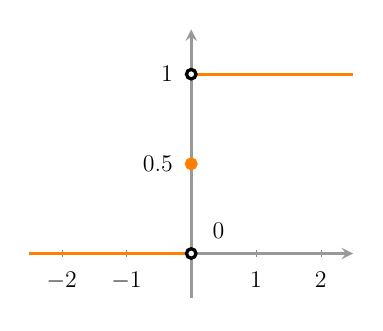
\begin{tikzpicture}[ scale=0.6,inner sep=0.8em ]

\tikzstyle{every path}=[line width=2pt]

\begin{axis}[axis lines=middle, draw=gray!80,
    ticklabel style = {font=\Large },
    xmin=-2.5, xmax=2.5,
    ymin=-0.25, ymax=1.25,
    %xtick=\empty,
     ytick={0.5,1},
     extra y ticks={0},
     extra y tick style={
       tick label style={anchor=south west, xshift=6pt},
     },
   % enlargelimits=true
]
\addplot[orange,smooth,domain=0:2.5] {1};
\addplot[orange,smooth,domain=-2.5:0] {0};
\draw[black,fill=white] (axis cs:0,0) circle(1mm)  (axis cs:0,1) circle(1mm);
\draw[fill,orange] (axis cs:0,1/2) circle(1mm);
\end{axis}
\end{tikzpicture}
\end{center}
\caption{Plot of the Heaviside step function  $H(x)$.
Its value at $x=0$ depends on its definition.}
\label{2011-m-fhsf}
\end{marginfigure}
Alternatively one may define $H(0)=\frac{1}{2}$, as plotted in Fig. \ref{2011-m-fhsf}.
\begin{equation}
H(x-x_0)
=   \frac{1}{2} + \frac{1}{\pi } \lim_{\varepsilon \rightarrow 0^+} \textrm{arctan}\left( \frac{x-x_0}{\varepsilon} \right)
=
\left\{
\begin{array}{rl}
1&\textrm{ for } x > x_0\\
\frac{1}{2}&\textrm{ for } x = x_0\\
0&\textrm{ for } x < x_0
\end{array}
\right.
\label{2012-m-di-hsfoh}
\end{equation}
and, since this affects only an isolated point at $x=x_0$, we may happily do so if we prefer.

It is also very common to define the  unit step function as the
{\em antiderivative  of the $\delta$ function};
\index{antiderivative}
likewise the delta function is the derivative of the Heaviside step function; that is,
\begin{equation}
\begin{split}
H'[\varphi ]=\delta [\varphi ]\text{, or formally,}\\
H(x-x_0)
=
\int_{-\infty}^{x-x_0} \delta (t) dt,\text{ and }
\frac{d}{dx} H(x-x_0)=\delta (x-x_0).
\end{split}
\end{equation}

{\color{OliveGreen}
\bproof
The latter equation can, in the functional sense -- that is, by integration over a test function --
be proven by
\begin{equation}
\begin{split}
H'[\varphi ]= \langle   H' , \varphi   \rangle = - \langle  H ,  \varphi'   \rangle
 =
-\int_{-\infty}^\infty H(x) \varphi' (x)  dx \\
 =
-\int_{0}^\infty  \varphi' (x)  dx
  =
-\left.   \varphi  (x) \right|_{x=0}^{x= \infty} \\
  =
 -   \underbrace{\varphi  (\infty)}_{=0} +  \varphi  (0)
  =    \langle   \delta , \varphi  \rangle  =\delta [\varphi ]
\end{split}
\end{equation}
for all test functions $\varphi (x)$. Hence we can -- in the functional sense  -- identify $\delta$ with $H'$.
More explicitly, through integration by parts, we obtain
\begin{equation}
\begin{split}
\int _{-\infty}^\infty \left[\frac{d}{dx} H(x-x_0)\right] \varphi (x) dx       \\
  =
\left. H(x-x_0) \varphi (x)\right| _{-\infty}^\infty - \int _{-\infty}^\infty H(x-x_0) \left[\frac{d}{dx} \varphi (x)\right] dx \\
  =
\underbrace{H(\infty)}_{=1}\underbrace{\varphi(\infty)}_{=0} - \underbrace{H(-\infty)}_{=0}\underbrace{\varphi(-\infty)}_{=0}
   - \int _{x_0}^\infty \left[\frac{d}{dx} \varphi (x)\right] dx  \\
 =  - \int _{x_0}^\infty \left[\frac{d}{dx} \varphi (x)\right] dx \\
 =    -  \left.  \varphi (x)   \right| _{x=x_0}^{x= \infty}
 =    - [  \underbrace{\varphi  (\infty)}_{=0}  - \varphi (x_0)]
 =     \varphi (x_0).
\end{split}
\end{equation}



\eproof
}

\subsection{Unit step function sequence}


As mentioned earlier, a commonly used limit form  of the Heaviside step function is
\begin{equation}
H(x)= \lim_{\epsilon \rightarrow 0} H_\epsilon (x)=\lim_{\epsilon \rightarrow 0}   \left[ \frac{1 }{2} + \frac{1 }{\pi} \tan^{-1}  \frac{x}{\epsilon } \right] .
\end{equation}
respectively.

Another limit representation of the Heaviside function is in terms of the
{\em Dirichlet's discontinuity factor} as follows:
\index{Dirichlet's discontinuity factor}
\begin{equation}
\begin{split}
H(x)= \lim_{t \rightarrow \infty} H_t (x)
\\
= \frac{1}{2}+\frac{1}{\pi }\lim_{t \rightarrow \infty}\int_0^t \frac{\sin (kx)}{k} dk
\\
=
\frac{1}{2}+\frac{1}{\pi }\int_0^\infty \frac{\sin (kx)}{k} dk
.
\end{split}
\label{2012-m-ch-di-dcf}
\end{equation}
%  Plot[(1/2) + (1/Pi)*Integrate[Sin[x*k]/k, {k, 0.001, 3*Pi}], {x, -3,  3}]

{\color{OliveGreen}
\bproof
A proof \cite{maor1998} uses a variant
of the {\em sine integral function}
\index{sine integral}
\begin{equation}
\textrm{Si}(y) = \int_0^y \frac{\sin t}{t} \,dt
\end{equation}
which in the limit of large argument $y$ converges towards
the {\em Dirichlet integral}   (no proof is given here)
\index{Dirichlet integral}
\begin{equation}
\lim_{y \rightarrow  \infty}\textrm{Si}(y) = \int_0^\infty  \frac{\sin t}{t} \,dt= \frac{\pi}{2}.
\label{2012-m-ch-di-diint}
\end{equation}


Suppose we
replace $t$ with $t=kx$
in the Dirichlet integral (\ref{2012-m-ch-di-diint}),
whereby $x\neq 0$ is a nonzero constant; that is,
\begin{equation}
\int_0^\infty  \frac{\sin (kx)}{kx} \,d(kx)
= H(x)\int_0^{\infty}  \frac{\sin (kx)}{k} \,dk
+H(-x)\int_0^{-\infty}  \frac{\sin (kx)}{k} \,dk
.
\label{2012-m-ch-di-diint2}
\end{equation}
Note that the integration border $\pm \infty$ changes, depending on whether $x$ is positive or negative,
respectively.

If $x$ is positive, we leave the integral
(\ref{2012-m-ch-di-diint2})
as is, and we recover the original Dirichlet integral (\ref{2012-m-ch-di-diint}),
which is $\frac{\pi}{2}$.
If $x$ is negative,
in order to recover the original Dirichlet integral form with the upper limit $\infty$,
we have to perform yet another substitution $k \rightarrow -k$
on (\ref{2012-m-ch-di-diint2}), resulting in
\begin{equation}
= \int_0^{-\infty}  \frac{\sin (-kx)}{-k} \,d(-k)
= -\int_0^{\infty}  \frac{\sin (kx)}{k} \,dk
= - \textrm{Si}(\infty ) =  -\frac{\pi}{2}
,
\label{2015-m-ch-di-diint3}
\end{equation}
since the sine function is an odd function; that is, $\sin(-\varphi )=-\sin \varphi $.


The Dirichlet's discontinuity factor (\ref{2012-m-ch-di-dcf})
is obtained by normalizing the absolute value of
(\ref{2012-m-ch-di-diint2}) [and thus also
(\ref{2015-m-ch-di-diint3})]
to $\frac{1}{2}$
by multiplying  it with $1/\pi$, and by adding $\frac{1}{2}$.
\eproof
}



\subsection{Useful formul\ae{} involving $H$}

Some other formul\ae{}  involving the unit step function
are
 \begin{equation}
H (-x)= 1-H(x)  \text{, or }   H(x) = 1 - H(-x),
 \end{equation}
 \begin{equation}
H (\pm x)=\lim_{\epsilon \rightarrow 0^+}{\mp i\over 2\pi
 }\int_{-\infty}^{+\infty} {e^{ikx}\over k\mp i\epsilon}dk,
 \end{equation}
and
 \begin{equation}
H (x)
={1\over 2}
+
\sum_{l=0}^\infty (-1)^l {(2l)!(4l+3)\over 2^{2l+2}l!(l+1)!}
P_{2l+1} (x),
 \end{equation}
where $P_{2l+1} (x)$ is a Legendre polynomial.
Furthermore,
\begin{equation}
\delta(x)=
\lim_{\varepsilon \rightarrow 0^+}  \frac{1}{\varepsilon } H\left( \frac{\varepsilon }{2} -\vert x\vert\right) .
\end{equation}
{\color{OliveGreen}
\bproof
The latter equation can
be proven by
\begin{equation}
\begin{split}
\lim_{\varepsilon \rightarrow 0^+}  \int_{-\infty}^\infty
\frac{1}{\varepsilon } H\left( \frac{\varepsilon }{2} -\vert x\vert\right) \varphi(x) dx
=
\lim_{\varepsilon \rightarrow 0^+} \frac{1}{\varepsilon } \int_{-\frac{\varepsilon}{2}}^{\frac{\varepsilon}{2}}
\varphi(x) dx
\\
\textrm{[mean value theorem: $\exists$  $y$ with $-\frac{\varepsilon}{2}\le y \le \frac{\varepsilon}{2}$ such that]} \\
=\lim_{\varepsilon \rightarrow 0^+} \frac{1}{\varepsilon }\varphi(y) \underbrace{\int_{-\frac{\varepsilon}{2}}^{\frac{\varepsilon}{2}} dx}_{=\varepsilon }
=\lim_{\varepsilon \rightarrow 0^+}  \varphi(y)  =   \varphi(0) =\delta [\varphi ].
\end{split}
\end{equation}
\eproof
}

An integral representation of $H(x)$ is
 \begin{equation}
H (x)
=\lim_{\epsilon \downarrow 0^+} \mp \frac{1}{2\pi i}
\int_{-\infty}^\infty
 \frac{1}{t \pm i\epsilon}e^{\mp ixt} dt.
 \end{equation}



\subsection{$H  \left[ \varphi \right]$ distribution}
The distribution associated with the Heaviside function $H(x)$ is defined by
\begin{equation}
H \left[ \varphi \right] =
\int_{-\infty}^\infty  H(x)  \varphi(x) dx.
 \end{equation}
$H  \left[ \varphi \right]$
can be evaluated and represented as follows:
\begin{equation}
\begin{split}
H  \left[ \varphi \right]
=
\int_{-\infty}^0  \underbrace{H(x)}_{=0} \varphi(x) dx
+
\int_{0}^\infty  \underbrace{H(x)}_{=1} \varphi(x) dx
=
\int_{0}^\infty      \varphi(x) dx
.
\end{split}
\end{equation}

\subsection{Regularized unit step function}
In order to be able to define the Fourier transformation
associated with the Heaviside function  we sometimes
consider the distribution of the {\em regularized Heaviside function}
\index{regularized Heaviside function}
\begin{equation}
H_\varepsilon (x) =H(x)e^{-\varepsilon x},
\label{2012-m-ch-di-rhfun}
\end{equation}
 with $\varepsilon >0$,
such that $\lim_{\varepsilon \rightarrow 0^+}  H_\varepsilon (x) =H (x)$.



\subsection{Fourier transform  of  the unit step function}
\index{Heaviside function}
\index{unit step function}

The Fourier transform of the Heaviside (unit step) function
cannot be directly obtained by insertion into Eq. (\ref{2011-m-efta1mg}), because the associated integrals do not exist.
\if01

{\color{OliveGreen}
\bproof
The following ``direct'' evaluation, making use of splitting up $\widetilde{H}(k)$ in its even and odd components,
should be understood in the  functional sense.
\begin{equation}
\begin{split}
 \widetilde{H}(k)
=   \int_{-\infty}^\infty  H(x) e^{-i{kx}} dx   \\
\qquad
=   \int_{0}^\infty   e^{-i{kx}} dx
;   \\
 \widetilde{H}(-k)
=   \int_{-\infty}^\infty  H(x) e^{+i{kx}} dx   \\
\qquad
=   \int_{0}^\infty  H(x) e^{+i{kx}} dx   \\
\textrm{ [variable transformation: }x\rightarrow -x \textrm{]}  \\
\qquad
=  - \int_0^{-\infty} e^{-i{kx}} dx   \\
\qquad
=   \int_{-\infty}^0 e^{-i{kx}} dx
.
\end{split}
\end{equation}
Now separate the even part $E$ from the odd part $O$ of $H$; that is, define
\begin{equation}
\begin{split}
E(k) = (\widetilde{H}(k) + \widetilde{H}(-k))\\
\qquad =   \int_{-\infty}^{+\infty} e^{-i{kx}} dx      \\
\qquad \; [\textrm{substitution } x\rightarrow -x]\\
\qquad =   -\int_{+\infty}^{-\infty} e^{ i{kx}} dx      \\
\qquad =    \int_{-\infty}^{+\infty} e^{ i{kx}} dx      \\
\qquad =    2\int_{0}^{+\infty} \cos (kx) dx      \\
\qquad =   2\pi \delta(k);      \\
O(k) = (\widetilde{H}(k) - \widetilde{H}(-k))\\
\qquad =   \int_{0}^\infty \left[  e^{-i{kx}}- e^{+i{kx}}\right]  dx ,   \\
\qquad =   -2 i \int_{0}^\infty \sin (kx)  dx    \\
\qquad =   - 2 i {\cal P} \frac{1}{k} ;    \\
\widetilde{H}(k) = \frac{1}{2}(E(k)+O(k)) \\
\qquad =     \int_{0}^{+\infty} \left[ \cos (kx) - i\sin (kx) \right] dx  \\
\qquad =    \pi \delta (k) - i{\cal P}\frac{1}{k}
.
\end{split}
\end{equation}
The two integrals defining $E$ and $O$
must be interpreted in the functional sense.




%http://www.mathkb.com/Uwe/Forum.aspx/math/12158/How-to-find-Fourier-Transform-for-special-functions-how-to-evaluate
% Daryl McCullough Ithaca, NY
\eproof
}
\fi
For a derivation of  the Fourier transform of the Heaviside (unit step) function
we shall thus use the  regularized Heaviside function (\ref{2012-m-ch-di-rhfun}), and arrive at
{\em Sokhotsky's  formula} (also known as the {\em Plemelj's  formula}, or the {\em Plemelj-Sokhotsky formula})
\index{Sokhotsky formula}
\index{Plemelj formula}
\index{Plemelj-Sokhotsky formula}
\begin{equation}
\begin{split}
 {\cal F}[H(x)]=\widetilde{H}(k)=   \int_{-\infty}^\infty  H(x) e^{-i{kx}} dx   \\
\qquad =    \pi \delta(k) -  i {\cal P}  \frac{1}{k} \\
\qquad =   -i \left(i\pi \delta(k) + {\cal P} \frac{1}{k}\right)\\
\qquad =   \lim_{\varepsilon \rightarrow 0^+} -\frac{i}{k-i\varepsilon }
\end{split}
\end{equation}

{\color{OliveGreen}
\bproof
We shall compute the Fourier transform of the regularized Heaviside function
$H_\varepsilon (x) =H(x)e^{-\varepsilon x}$, with $\varepsilon >0$, of Eq. (\ref{2012-m-ch-di-rhfun}); that is  \cite{sommer-di},
\begin{equation}
\begin{split}
 {\cal F}[H_\varepsilon (x)] =
 {\cal F}[H(x)e^{-\varepsilon x}]
=\widetilde{H_\varepsilon }(k)
\\
=   \int_{-\infty}^\infty  H_\varepsilon (x) e^{-i{kx}} dx
\\
=   \int_{-\infty}^\infty  H(x)e^{-\varepsilon x}  e^{-i{kx}} dx
\\
=   \int_{-\infty}^\infty  H(x) e^{-i{kx}+(-i)^2\varepsilon x}  dx
\\
=   \int_{-\infty}^\infty  H(x) e^{-i(k - i \varepsilon ) x}  dx
\\
=   \int_{0}^\infty  e^{-i(k - i \varepsilon ) x}  dx
\\
=  \left. \left[ -\frac{ e^{-i(k - i \varepsilon ) x}}{i(k - i \varepsilon ) } \right] \right|_{x=0}^{x=\infty}
=  \left. \left[ -\frac{ e^{-ik} e^{- \varepsilon   x}}{i(k - i \varepsilon ) } \right] \right|_{x=0}^{x=\infty}
\\
=  \left[ -\frac{ e^{-ik\infty} e^{- \varepsilon  \infty}}{i(k - i \varepsilon ) } \right]
-  \left[ -\frac{ e^{-ik0} e^{- \varepsilon  0}}{i(k - i \varepsilon ) } \right]
\\
=    0 - \frac{ (-1)}{i(k - i \varepsilon ) }
=     -\frac{ i}{k - i \varepsilon  }
= -i \left[ {\cal P} \left(\frac{1}{k}\right) + i \pi \delta (k)  \right]
.
\end{split}
\end{equation}
where in the last step Sokhotsky's  formula~(\ref{2012-m-ch-di-Sokhotskyformula2})
has been used.
We therefore conclude that
\begin{equation}
 {\cal F}[H(x)] =
 {\cal F}[H_{0^+} (x)] =
 \lim_{\varepsilon \rightarrow 0^+} {\cal F}[H_\varepsilon (x)] =
  \pi \delta (k)   -i {\cal P} \left(\frac{1}{k}\right)
.
\label{2012-m-ch-di-fthfu}
\end{equation}

\eproof
}



%%%%%%%%%%%%%%%%%%%%%%%%%%%%%%%%%%%%%%%%%%%%%%%%%%%%%%%% sign function

\section{The sign function}

\subsection{Definition}
The
{\em sign function}
\index{sign function}
is defined by
\begin{equation}
\begin{split}
\textrm{sgn}(x-x_0)
=
\lim_{\varepsilon \rightarrow 0^+}
\frac{2}{\pi}
\textrm{arctan}\left( \frac{x-x_0}{\varepsilon } \right)
=
\left\{
\begin{array}{rl}
-1&\textrm{ for } x < x_0\\
0&\textrm{ for } x = x_0 \\
+1&\textrm{ for } x > x_0
\end{array}
\right.
.
\end{split}
\end{equation}
It is plotted in Fig. \ref{2011-m-fsf}.
\begin{marginfigure}
\begin{center}
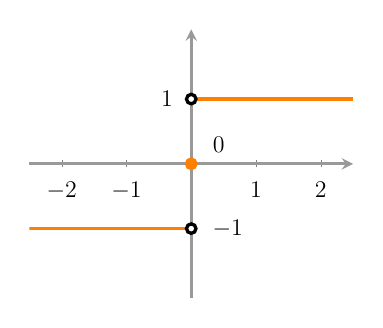
\begin{tikzpicture}[ scale=0.6,inner sep=0.8em]

\tikzstyle{every path}=[line width=2pt]


\begin{axis}[
axis lines=middle,axis equal,
    ticklabel style = {font=\Large },
    draw=gray!80,
    xmin=-2.5, xmax=2.5,
    ymin=-1.5, ymax=1.5,
     %xtick=\empty,
     extra x ticks={0},
     extra x tick style={tick label style={anchor=south west, xshift=4pt}},
     ytick={0,1},
     extra y ticks={-1},
     extra y tick style={tick label style={anchor=west, xshift=6pt}}
   % enlargelimits=true
]

\addplot[orange,smooth,domain=0:2.5] {1};
\addplot[orange,smooth,domain=-2.5:0] {-1};
\draw[black,fill=white] (axis cs:0,-1) circle(1mm)  (axis cs:0,1) circle(1mm);
\draw[fill,orange] (axis cs:0,0) circle(1mm);

\end{axis}
\end{tikzpicture}
\end{center}
\caption{Plot of the sign function.}
\label{2011-m-fsf}
\end{marginfigure}

\subsection{Connection to the Heaviside function}

In terms of  the  Heaviside step function, in particular, with
$H(0)=\frac{1}{2}$ as in Eq. (\ref{2012-m-di-hsfoh}),
the sign function can be written by ``stretching'' the former (the Heaviside step function) by a factor of two,
and shifting it by one negative unit as follows
\begin{equation}
\begin{split}
\textrm{sgn}(x-x_0) = 2H(x-x_0) -1,\\
H(x-x_0) = \frac{1}{2} \left[ \textrm{sgn}(x-x_0)+1\right];  \\
\textrm{and also}\\
\textrm{sgn}(x-x_0) = H(x-x_0) - H(x_0-x).
\end{split}
\label{2011-m-cbhsf}
\end{equation}
Therefore, the derivative of the sign function is
\begin{equation}
\frac{d}{dx}\textrm{sgn}(x-x_0) = \frac{d}{dx} \left[2H(x-x_0) -1\right] =2 \delta(x-x_0).
\end{equation}

Note also that  $\textrm{sgn}(x-x_0) =  - \textrm{sgn}(x_0-x)$.

\subsection{Sign sequence}


%http://home.comcast.net/~szemengtan/LinearSystems/fourier.pdf
The sequence of functions
\begin{equation}
\begin{split}
\textrm{sgn}_n(x-x_0)
=
\left\{
\begin{array}{rl}
- e^{-\frac{x}{n}}&\textrm{ for } x < x_0\\
+ e^{\frac{-x}{n}}&\textrm{ for } x > x_0
\end{array}
\right.
\end{split}
\label{2012-m-ch-di-lsegn}
\end{equation}
is a limiting sequence of
$
\textrm{sgn}(x-x_0)\stackrel{x\neq x_0}{=} \lim_{n\rightarrow \infty} \textrm{sgn}_n(x-x_0)
$.


We can also use the Dirichlet integral
\index{Dirichlet integral}
to express a limiting sequence for the sign function,
in a similar way as the derivation of Eqs.~(\ref{2012-m-ch-di-dcf}); that is,
\begin{equation}
\begin{split}
\textrm{sgn}(x)= \lim_{t \rightarrow \infty} \textrm{sgn}_t (x)
\\
= \frac{2}{\pi }\lim_{t \rightarrow \infty}\int_0^t \frac{\sin (kx)}{k} dk
\\
=
\frac{2}{\pi }\int_0^\infty \frac{\sin (kx)}{k} dk
.
\end{split}
\label{2015-m-ch-di-sign}
\end{equation}
%  Plot[(2/Pi)*Integrate[Sin[x*k]/k, {k, 0.001, 3*Pi}], {x, -3,  3}]

Note (without proof) that
\begin{eqnarray}
\mbox{sgn}(x)
&=&{4\over \pi }\sum_{n=0}^\infty {\sin [
(2n+1)x]\over
(2n+1)}\\
&=&{4\over \pi }\sum_{n=0}^\infty (-1)^n{\cos [
(2n+1)(x-\pi /2)]\over
(2n+1)}\;,\; -\pi <x<\pi  .
 \end{eqnarray}




\subsection{Fourier transform of $\textrm{sgn}$}

Since the Fourier transform is linear,
we may use the connection between the sign and the Heaviside functions $\textrm{sgn}(x) = 2H(x) -1$, Eq. (\ref{2011-m-cbhsf}),
together with the
Fourier transform of the Heaviside function
${\cal F}[H(x)] =  \pi \delta (k)   -i {\cal P} \left(\frac{1}{k}\right)$,
Eq. (\ref{2012-m-ch-di-fthfu}) and the Dirac delta function
${\cal F}[1] = 2\pi \delta (k)$, Eq. (\ref{2011-m-eftdelta1}),
to compose and compute the Fourier transform  of $\textrm{sgn}$:
\begin{equation}
\begin{split}
{\cal F}[\textrm{sgn}(x)] = {\cal F}[2H(x) -1] = 2{\cal F}[H(x)] - {\cal F}[1]
\\ \qquad =
2 \left[\pi \delta (k)   -i {\cal P} \left(\frac{1}{k}\right)\right] -  2\pi \delta (k)
\\ \qquad =
-2i {\cal P} \left(\frac{1}{k}\right)
.
\end{split}
\label{2011-m-ch-di-fdsgnfu}
\end{equation}

\if01
We shall consider the Fourier transform of the limit of the sequence (\ref{2012-m-ch-di-lsegn})
and assume (without proof) that, in the functional sense,
this yields the   Fourier transform of $\textrm{sgn}$; that is,
$
\lim_{n\rightarrow \infty}
{\cal F}[ \textrm{sgn}_n(x) ]
=
{\cal F}[ \textrm{sgn}(x) ]
$.

So, consider
%\marginpar{{\small http://www.eee.hku.hk/~work8501/WWW2008/ho3.pdf}}
\begin{equation}
\begin{split}
  {\cal F}[\textrm{sgn}_n (x)]= \int_{-\infty}^\infty  \textrm{sgn}_n (x) e^{-i{kx}} dx   \\
\qquad =
\int_{0}^\infty  e^{-\frac{x}{n}} e^{-i{kx}} dx
-
\int_{-\infty}^0  e^{ \frac{x}{n}} e^{-i{kx}} dx
\\
\qquad =
\int_{0}^\infty  e^{-\left(\frac{1}{n}+i{k}\right) x} dx
-
\int_{-\infty}^0  e^{ \left(\frac{1}{n}-i{k}\right) x} dx
\\
\qquad \;
[\textrm{substitution }x \rightarrow -x \textrm{ in second integral}]\\
\qquad =
\int_{0}^\infty  e^{-\left(\frac{1}{n}+i{k}\right) x} dx
-
\int_{0}^\infty  e^{-\left(\frac{1}{n}-i{k}\right) x} dx
\\
\qquad =
\left.  \frac{ e^{-\left(\frac{1}{n}+i{k}\right) x}}{{-\left(\frac{1}{n}+i{k}\right)  }} \right|_{0}^\infty
-
\left.  \frac{ e^{-\left(\frac{1}{n}-i{k}\right) x}}{-\left(\frac{1}{n}-i{k}\right)} \right|_{0}^\infty
\\
\qquad =
  \frac{ 1}{  \frac{1}{n}+i{k} }
-
 \frac{ 1 }{ \frac{1}{n}-i{k} }
.
\end{split}
\label{2011-m-ftsgn1a}
\end{equation}
Thus,
\begin{equation}
\begin{split}
{\cal F}[\textrm{sgn}  (x)] =\lim_{n\rightarrow \infty}  {\cal F}[\textrm{sgn}_n (x)]
\\
\qquad =  \lim_{n\rightarrow \infty}  \left(
  \frac{ 1}{ \frac{1}{n}+i{k}   }
-
 \frac{ 1 }{  \frac{1}{n}-i{k}   }          \right)
\\
\qquad =
  \frac{ 1}{   i{k}  }
+
 \frac{ 1 }{  i{k} }
 =
  -\frac{2i}{ k }
.
\end{split}
\label{2011-m-ftsgn1b}
\end{equation}
\fi


%%%%%%%%%%%%%%%%%%%%%%%%%%%%%%%%%%%% absolute value function



\section{Absolute value function (or modulus)}
\index{absolute value}
\index{modulus}

\subsection{Definition}
The {\em absolute value} (or {\em modulus})
of $x$ is defined by
\begin{equation}
\left|
x-x_0\right|
=
\left\{
\begin{array}{ll}
x-x_0&\textrm{ for } x > x_0\\
0&\textrm{ for } x = x_0\\
x_0-x&\textrm{ for } x < x_0
\end{array}
\right.
\label{2011-m-di-avm}
\end{equation}
It is plotted in Fig. \ref{2011-m-avm}.
\begin{marginfigure}
\begin{center}
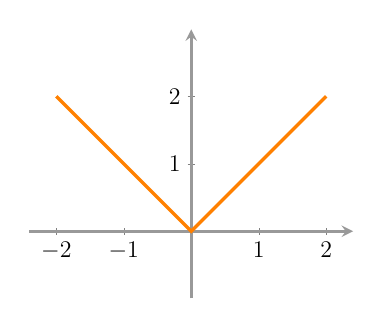
\begin{tikzpicture}[ scale=0.6,
 declare function={
    func(\x)= (\x <= 0) * (-\x)   +
             % and(\x >= -1,\x <= 1) * (exp(1/( \x*\x-1)))     +
              (\x > 0) * (\x)
   ;
                  } ]

\tikzstyle{every path}=[line width=2pt]

\begin{axis}[axis lines=middle,
draw=gray!80,
enlargelimits=true,axis equal,
ticklabel style = {font=\Large },
]
\addplot [
orange,
domain=-2:2,
%samples=201,
line width=3pt
]  {func(x)};
\end{axis}
\end{tikzpicture}
\caption{Plot of the absolute value function $f(x)=\left|x\right|$.}
\label{2011-m-avm}
\end{center}
\end{marginfigure}

\subsection{Connection of absolute value with the sign and Heaviside functions}

Its relationship to the sign function is twofold:
on the one hand, there is
 \begin{equation}
 \left|x\right| = x \,\textrm{sgn} (x),
 \end{equation}
and thus, for $x\neq 0$,
 \begin{equation}
\textrm{sgn} (x)  = \frac{\left|x\right|}{x} = \frac{x}{\left|x\right|}.
 \end{equation}

On the other hand, the derivative of the absolute value function is the sign function, at least up to a singular point at $x=0$,
and thus the absolute value function can be interpreted as the integral of the sign function (in the distributional sense);
that is,
\begin{equation}
\begin{split}
\frac{d}{dx} \left|x\right| \left[ \varphi \right]
=
\textrm{sgn}\left[ \varphi \right] \text{, or, formally,}
\\
\frac{d }{dx} \left|x\right|
=
\textrm{sgn} (x)
=
\left\{
\begin{array}{rl}
1&\textrm{ for } x > 0\\
0&\textrm{ for } x = 0\\
-1&\textrm{ for } x < 0
\end{array}
\right.
,\\
\text{and } \left|x\right| =  \int \textrm{sgn} (x) dx.
\end{split}
 \end{equation}

{\color{OliveGreen}
\bproof
This can  be formally proven by inserting
$\left|x\right|  =  {x}\, \textrm{sgn} (x)$; that is,
\begin{equation}
\begin{split}
\frac{d }{dx}  \left|x\right|
=
\frac{d }{dx}x\,\textrm{sgn} (x)
=
\textrm{sgn} (x)  + x\frac{d}{dx} \textrm{sgn} (x)
\\
=
\textrm{sgn} (x)  + x\frac{d }{dx}\left[2H(x)-1\right]
=
\textrm{sgn} (x) - 2\underbrace{x\delta(x)}_{=0}.
\end{split}
 \end{equation}

Another proof is via linear functionals:
\begin{equation}
\begin{split}
\frac{d }{dx}  \left|x\right|   \left[ \varphi \right]
= -  \left|x\right|   \left[ \varphi' \right]
= -\int_{-\infty}^\infty  \left|x\right|   \varphi'  (x) dx
\\
= -\int_{-\infty}^0 \underbrace{\left|x\right|}_{=-x}   \varphi'  (x) dx
- \int_{0}^\infty  \underbrace{\left|x\right|}_{=x}    \varphi'  (x) dx
\\
= \int_{-\infty}^0  x    \varphi'  (x) dx - \int_{0}^\infty   x    \varphi'  (x) dx
\\
= \underbrace{\left. x \varphi   (x)\right|_{-\infty}^0}_{=0}  -  \int_{-\infty}^0    \varphi   (x) dx  -  \underbrace{\left. x \varphi   (x)\right|_0^{\infty}}_{=0}  + \int_{0}^\infty        \varphi'  (x) dx
\\
=   \int_{-\infty}^0    (-1) \varphi   (x) dx      + \int_{0}^\infty  (+1)    \varphi'  (x) dx  \\
=   \int_{-\infty}^\infty     \textrm{sgn}(x) \varphi   (x) dx
= \textrm{sgn}\left[ \varphi \right]
.
\end{split}
 \end{equation}


\eproof
}



\section{Some examples}

{
\color{blue}
\bexample

Let us compute some concrete examples related to distributions.
\begin{enumerate}
\item
For a start, let us prove that
\begin{equation}
\lim_{\epsilon \rightarrow 0}{\epsilon \sin^2 \frac{x}{\epsilon}\over \pi
 x^2}= \delta (x).\end{equation}
As a hint, take  $\int_{-\infty}^{+\infty} {\sin^2x\over x^2}dx =\pi $.

Let us prove this conjecture by integrating over a good test function $\varphi$
\begin{equation}
\begin{split}
   {1\over\pi}\lim_{\epsilon \rightarrow 0}\int\limits_{-\infty}^{+\infty}
   {\varepsilon\sin^2\left({x\over\varepsilon}\right)\over x^2} \varphi(x) dx
\\
 \textrm{[variable substitution}\;   y={x\over\varepsilon} , {dy\over dx}={1\over\varepsilon}, dx=\varepsilon dy
\textrm{]}
\\  =
  {1\over\pi}\lim_{\epsilon \rightarrow 0}
   \int\limits_{-\infty}^{+\infty}\varphi(\varepsilon y)
   {\varepsilon^2\sin^2(y)\over \varepsilon^2y^2}dy
\\  =    {1\over\pi}
   \varphi(0)\int\limits_{-\infty}^{+\infty}{\sin^2(y)\over y^2}dy
  =    \varphi(0).
\end{split}
\end{equation}
Hence we can identify
\begin{equation}
   \lim_{\varepsilon \rightarrow 0}{\varepsilon\sin^2 \left({x\over\varepsilon}\right)\over\pi x^2}=\delta(x).
\end{equation}

 \item
In order to prove that $\frac{1}{\pi} \frac{n  e^{-x^2}}{1+n^2x^2} $ is  a  $\delta$-sequence
we proceed again by integrating over a good test function $\varphi$,
and with the hint that $\int\limits_{-\infty}^{+\infty} dx/ (1+x^2) =\pi$ we obtain
 \begin{equation}
\begin{split}
\lim_{n \rightarrow \infty}  \frac{1}{\pi}
\int\limits_{-\infty}^{+\infty}
\frac{n  e^{-x^2}}{1+n^2x^2}
   \varphi(x)
dx
\\  \textrm{[variable substitution }    y={xn} , x={y\over n}, {dy\over dx}={n}, dx={dy\over n}
\textrm{]}
\\   =
\lim_{n \rightarrow \infty}   \frac{1}{\pi}
\int\limits_{-\infty}^{+\infty}
\frac{n  e^{-\left( \frac{y}{n} \right)^2}}{1+y^2}
   \varphi \left( \frac{y}{n} \right)
\frac{dy}{n}
\\  =
\frac{1}{\pi}
\int\limits_{-\infty}^{+\infty}
\lim_{n \rightarrow \infty}  \left[     e^{-\left( \frac{y}{n} \right)^2}  \varphi \left( \frac{y}{n} \right) \right]
\frac{1}{1+y^2}
dy
\\   =       \frac{1}{\pi}
\int\limits_{-\infty}^{+\infty}
\left[     e^{0}  \varphi \left( 0\right) \right]
\frac{1}{1+y^2}
dy
\\   =    \frac{\varphi \left( 0\right)}{\pi}
\int\limits_{-\infty}^{+\infty}
\frac{1}{1+y^2}
dy   =
\frac{\varphi \left( 0\right)}{\pi} \pi
   =
\varphi \left( 0\right).
\end{split}
\end{equation}
Hence we can identify
\begin{equation}
   \lim_{n \rightarrow \infty}{\frac{1}{\pi} \frac{n  e^{-x^2}}{1+n^2x^2}}=\delta(x).
\end{equation}

\item
Let us prove that
$x^n\delta^{(n)}[\varphi]=C\delta [\varphi]$    and determine the constant $C$.
We proceed again by integrating over a good test function $\varphi$.
First note that if
$\varphi (x)$ is a good test function, then so is
$x^n\varphi (x)$.
 \begin{equation}
\begin{split}
    x^n\delta^{(n)}[\varphi] =
   \int dx x^n\delta^{(n)}(x)\varphi(x) \\  =
   \int dx \delta^{(n)}(x)\bigl[x^n\varphi(x)\bigr]=
   =(-1)^n \int dx \delta(x)\bigl[x^n\varphi(x)\bigr]^{(n)}=\\
  =(-1)^n \int dx \delta(x)\bigl[nx^{n-1}\varphi(x)+x^n\varphi'(x)
   \bigr]^{(n-1)}=
 \cdots \\
   =(-1)^n \int dx \delta(x)\left[\sum_{k=0}^n
           \left(
          \begin{array}{c}
          n\\ k
           \end{array}\right) (x^n)^{(n-k)}\varphi ^{(k)}(x)\right]
    \\
   =(-1)^n \int dx
\delta(x)\bigl[n!\varphi(x)+n\cdot n!x\varphi'(x) +
\cdots +x^n\varphi^{(n)}(x)
   \bigr] \\
   =(-1)^n n! \int dx \delta(x)\varphi(x)
   =(-1)^n n!  \delta[\varphi ]
,
\end{split}
\end{equation}
and hence  $ C=(-1)^n n!$.


\item
Let us simplify $\int_{-\infty}^\infty \delta (x^2-a^2)g(x)\; dx$.
First recall Eq. (\ref{2011-m-distdp1})  stating that
$$
   \delta(f(x))=\sum_{i}{\delta(x-x_i)\over|f'(x_i)|},
$$
whenever $x_i$ are simple roots of  $f(x)$, and $f'(x_i)\neq 0$.
In our case, $
   f(x)=x^2-a^2=(x-a)(x+a)
$, and the roots are  $x=\pm a$.
Furthermore,
$
   f'(x)=(x-a)+(x+a)= 2x
$; therefore
$
   |f'(a)|=|f'(-a)|=2|a|$.
As a result,
$$
    \delta(x^2-a^2)=\delta\bigl((x-a)(x+a)\bigr)={1\over|2a|}
   \bigl(\delta(x-a)+\delta(x+a)\bigr).
$$
Taking this into account we finally obtain
 \begin{equation}
\begin{split}
  \int\limits_{-\infty}^{+\infty}\delta(x^2-a^2)
   g(x)dx\\
\qquad =
\int\limits_{-\infty}^{+\infty}{\delta(x-a)+\delta(x+a)\over
   2|a|}g(x)dx\\
\qquad =    {g(a)+g(-a)\over2|a|}.
\end{split}
\end{equation}


\item
Let us evaluate
\begin{equation}
I=
\int_{-\infty}^\infty
\int_{-\infty}^\infty
\int_{-\infty}^\infty
\delta (x_1^2+x_2^2+x_3^2-R^2) d^3x
\end{equation}
for  $R \in {\Bbb R}, R >0 $.
We may, of course, retain the standard Cartesian coordinate system and evaluate the integral by ``brute force.''
Alternatively,
a more elegant way is to use the spherical symmetry of the problem and use spherical coordinates $r, \Omega (\theta ,\varphi )$ by rewriting $I$
into
\begin{equation}
I=  \int_{r,\Omega} r^2  \delta (r^2-R^2) d\Omega dr.
\end{equation}
As the integral kernel $\delta (r^2-R^2)$ just depends on the radial coordinate $r$
the angular coordinates just integrate to $4\pi$.
Next we make use of Eq. (\ref{2011-m-distdp1}), eliminate the solution for $r=-R$, and obtain
\begin{equation}
\begin{split}
I= 4\pi   \int_0^\infty r^2  \delta (r^2-R^2)  dr \\
 =  4\pi   \int_0^\infty  r^2 \frac{\delta (r+R) + \delta (r-R)}{2R}  dr \\
  =   4\pi   \int_0^\infty  r^2 \frac{\delta (r-R)}{2R}  dr \\
  =   2 \pi R.
\end{split}
\end{equation}

\item
Let us compute
\begin{equation}
\int_{-\infty}^\infty \int_{-\infty}^\infty  \delta
 (x^3-y^2+2y)\delta (x+y)H (y-x-6)f(x,y) \,dx\,dy.
\end{equation}

First, in dealing with
$\delta(x+y)$, we evaluate the $y$ integration at $x=-y$ or $y=-x$:
$$
   \int_{-\infty}^\infty \delta(x^3-x^2-2x)H(-2x-6)f(x,-x)  dx
$$
Use of Eq. (\ref{2011-m-distdp1})
$$
   \delta(f(x))=\sum_{i}{1\over|f'(x_i)|}\delta(x-x_i),
$$
at the roots
\begin{equation}
\begin{split}
   x_1=0\\
   x_{2,3}={1\pm\sqrt{1+8}\over 2}={1\pm3\over2}=\left\{{2\atop-1}\right.
\end{split}
\end{equation}
of the argument $f(x)=x^3-x^2-2x=x(x^2-x-2)=x(x-2)(x+1)$ of the remaining $\delta$-function,
together with
$$
 f'(x)=  {d\over dx}(x^3-x^2-2x)=3x^2-2x-2 ;
$$
yields
\begin{equation}
\begin{split}
   \int\limits_{-\infty}^\infty dx
         {\delta(x)+\delta(x-2)+\delta(x+1)\over|3x^2-2x-2|}
         H(-2x-6)f(x,-x \\
   ={1\over|-2|}\underbrace{H(-6)}_{ =0 }f(0,-0)+
      {1\over|12-4-2|}\underbrace{H(-4-6)}_{ =0 }f(2,-2)  +\\
   +\ {1\over|3+2-2|}\underbrace{H(2-6)}_{ =0 }f(-1,1)
=0
\end{split}
\end{equation}


\item
When simplifying derivatives of generalized functions it is always useful to evaluate their properties
--
such as $x\delta(x)=0$, $f(x)\delta(x-x_0)=f(x_0)\delta(x-x_0)$, or $\delta (-x)=\delta (x)$
--
first and  before proceeding with the next differentiation or evaluation.
We shall present some applications of this ``rule'' next.

First, simplify
\begin{equation}
\left({d\over dx}-\omega \right)H (x)e^{\omega x}
\end{equation}
as follows
\begin{equation}
\begin{split}
 {d\over dx}\left[H(x)e^{\omega
x}\right]-\omega H(x)e^{\omega x}\\
\qquad =
   \delta(x)e^{\omega x}+\omega H(x)e^{\omega x}-\omega H(x)
   e^{\omega x}\\
\qquad =
   \delta(x)e^{0}
   \\
\qquad =  \delta(x)
\end{split}
\end{equation}


\item
Next, simplify
\begin{equation}
\left({d^2\over dx^2}+\omega^2 \right){1\over \omega }H
 (x)\sin (\omega x)
\end{equation}
as follows
\begin{equation}
\begin{split}
{d^2\over dx^2}\left[{1\over\omega}H(x)\sin(\omega
x)\right]+\omega H(x)
      \sin(\omega x)\\
   \qquad =   {1\over\omega}{d\over dx}\Bigl[\underbrace{\delta(x)\sin(\omega x)}_
      {\mbox{$=0$}}+\omega H(x)\cos(\omega x)\Bigr]+\omega H(x)
      \sin(\omega x)\\
  \qquad =   {1\over\omega}\Bigl[\omega\underbrace{\delta(x)\cos(\omega x)}_
      {\mbox{$\delta(x)$}}-\omega^2H(x)\sin(\omega x)\Bigr]+
      \omega H(x)\sin(\omega x)=\delta(x)
\end{split}
\end{equation}

\begin{marginfigure}
{\color{black}
\begin{center}
\begin{tabular}{c}

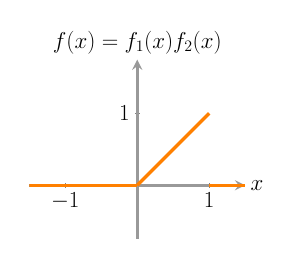
\begin{tikzpicture}[ scale=0.4,
 declare function={
    func(\x)= (\x )
   ;
                  } ]

\tikzstyle{every path}=[line width=3pt]

\begin{axis}[axis lines=middle, draw=gray!80,
%enlargelimits=true,
axis equal,
xtick={-1,0,1},
ytick={-1,0,1},
ticklabel style = {font=\huge },
every axis x label/.style={
    at={(ticklabel* cs:1)},
    anchor=west,
    font=\huge ,
},
every axis y label/.style={
    at={(ticklabel* cs:1)},
    anchor=south,
    font=\huge ,
},
xlabel={$x$},
ylabel={$f(x)=f_1(x)f_2(x)$}
]

\addplot[orange,line width=2pt,smooth,domain=-1.5:0] {0};
\addplot [
orange,
domain=0:1,
%samples=201,
line width=3pt
]  {func(x)};
\addplot[orange,line width=2pt,smooth,domain=1:1.5] {0};


\end{axis}
\end{tikzpicture}
\\
(a) $\,$\\
\\
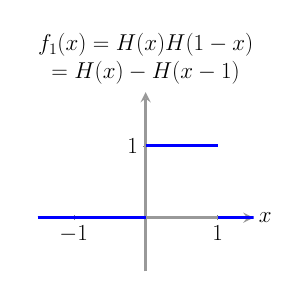
\begin{tikzpicture}[ scale=0.4,
 declare function={
    func(\x)= (\x <= 0) * (0)   +
              and(\x >= 0,\x <= 1) * ( 1 )     +
              (\x > 1) * (0 )
   ;
                  } ]

\tikzstyle{every path}=[line width=3pt]

\begin{axis}[axis lines=middle, draw=gray!80,
%enlargelimits=true,
axis equal,
xtick={-1,0,1},
ytick={-1,0,1},
ticklabel style = {font=\huge },
every axis x label/.style={
    at={(ticklabel* cs:1)},
    anchor=west,
    font=\huge ,
},
every axis y label/.style={
    at={(ticklabel* cs:1)},
    anchor=south,
    font=\huge ,
},
xlabel={$x$},
ylabel={\begin{tabular}{c}$f_1(x)=H(x)H(1-x)$\\$=H(x)- H(x-1)$\end{tabular}}
]

\addplot[blue,line width=2pt,smooth,domain=-1.5:0] {0};
\addplot[blue,line width=2pt,smooth,domain=0:1] {1};
\addplot[blue,line width=2pt,smooth,domain=1:1.5] {0};


\end{axis}
\end{tikzpicture}
\\
(b) $\,$\\
\\
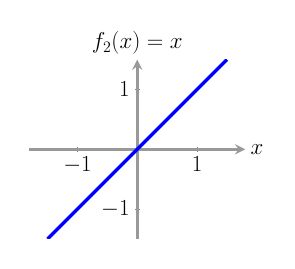
\begin{tikzpicture}[ scale=0.4,
 declare function={
    func(\x)= (\x <= 0) * (\x)   +
             % and(\x >= -1,\x <= 1) * (exp(1/( \x*\x-1)))     +
              (\x > 0) * (\x)
   ;
                  } ]

\tikzstyle{every path}=[line width=3pt]

\begin{axis}[axis lines=middle, draw=gray!80,axis equal,
xtick={-1,0,1},
ytick={-1,0,1},
ticklabel style = {font=\huge },
every axis x label/.style={
    at={(ticklabel* cs:1)},
    anchor=west,
    font=\huge ,
},
every axis y label/.style={
    at={(ticklabel* cs:1)},
    anchor=south,
    font=\huge ,
},
xlabel={$x$},
ylabel={$f_2(x)=x$}
]
\addplot [
blue,
domain=-1.5:1.5,
samples=201,
line width=3pt
]  {func(x)};
\end{axis}
\end{tikzpicture}
\\
(c)
\end{tabular}
\end{center}
}
\caption{Composition of
$f (x)=f_1(x)f_2(x)$.
}
\label{2011-m-fcof1}
\end{marginfigure}

\item
Let us compute the $n$th derivative of
\begin{equation}
f (x)
=
\begin{cases}
0  & \textrm{ for }    x< 0 ,\\
x  & \textrm{ for }   0\le x\le 1, \\
0  &\textrm{ for }  x>1.
\end{cases}
\end{equation}



As depicted in Fig. \ref{2011-m-fcof1},
$f$ can be composed from two functions $f(x)=f_2(x)\cdot f_1(x)$;
and this composition can be done in at least two ways.


Decomposition {(i)} yields
\begin{equation}
\begin{split}
   f(x)=x\bigl[H(x)-H(x-1)\bigr]=xH(x)-xH(x-1)\\
   f'(x)=H(x)+\underbrace{x\delta(x)}_{=0}-H(x-1)-x\delta(x-1)
\end{split}
\end{equation}
Because of $x\delta(x-a)=a\delta(x-a)$,
\begin{equation}
\begin{split}
   f'(x)=H(x)-H(x-1)-\delta(x-1)\\
   f''(x)=\delta(x)-\delta(x-1)-\delta'(x-1)
\end{split}
\end{equation}
and hence   by induction, for $n>1$,
\begin{equation}
f^{(n)}(x)=\delta^{(n-2)}(x)-\delta^{(n-2)}(x-1)-   \delta^{(n-1)}(x-1)
.
\end{equation}

Decomposition {(ii)}  yields the same result as  decomposition {(i)}, namely
\begin{equation}
\begin{split}
   f(x)=xH(x)H(1-x)\\
   f'(x)=H(x)H(1-x)+         \underbrace{x\delta(x)}_{ =0 } H(1-x)+\underbrace{xH(x)(-1)\delta(1-x)}_{=-H(x)\delta(1-x)}\\
   =H(x)H(1-x) - \delta(1-x)\\
\text{[with $\delta(x)=\delta(-x)$]}  =        H(x)H(1-x) - \delta(x-1)\\
   f''(x)=\underbrace{\delta(x)H(1-x)}_{ =\delta(x) }         +\underbrace{(-1)H(x)\delta(1-x)}_{ -\delta(1-x) }        -\delta'(x-1) \\
        =\delta(x)-\delta(x-1)-\delta'(x-1);
\end{split}
\end{equation}
and hence   by induction, for $n>1$,
\begin{equation}
f^{(n)}(x)=\delta^{(n-2)}(x)-\delta^{(n-2)}(x-1)-
   \delta^{(n-1)}(x-1)
.
\end{equation}


\item
Let us compute the $n$th derivative of
 \begin{equation}
f (x)
=
\begin{cases}
\vert \sin x\vert & \textrm{ for } -\pi \le x\le \pi ,\\
 0  & \textrm{ for }  \vert x\vert >\pi .
\end{cases}
\end{equation}

$$
   f(x)=|\sin x|H(\pi+x)H(\pi-x)
$$
$$
   |\sin x|=\sin x\mbox{ sgn}(\sin x)=\sin x\mbox{ sgn\,}x\qquad\mbox{for}
   \quad -\pi<x<\pi ;
$$
hence we start from
$$
  f(x)=\sin x\mbox{ sgn\,}xH(\pi+x)H(\pi-x),
$$
Note that
\begin{eqnarray*}
   \mbox{ sgn\,}x&=&H(x)-H(-x),\\
   (\mbox{ sgn\,}x)'&=&H'(x)-H'(-x)(-1)=\delta(x)+\delta(-x)=
                   \delta(x)+\delta(x)=2\delta(x).
\end{eqnarray*}
\begin{eqnarray*}
   f'(x)   &=   &\cos x\mbox{ sgn\,}xH(\pi+x)
           H(\pi-x)+\sin x2\delta(x)H(\pi+x)H(\pi-x)+\\
           &    &+\sin x\mbox{ sgn\,}x\delta(\pi+x)H(\pi-x) +
           \sin x\mbox{ sgn\,}x H(\pi+x)\delta(\pi-x)(-1)=\\
           &=   &\cos x\mbox{ sgn\,}xH(\pi+x)H(\pi-x)\\
   f''(x)   &=   & -\sin x\mbox{ sgn\,}xH(\pi+x)H(\pi-x)+
             \cos x2\delta(x)H(\pi+x)H(\pi-x)+\\
           &    &+\cos x\mbox{ sgn\,}x\delta(\pi + x)H(\pi - x)
              + \cos x\mbox{ sgn\,}x H(\pi + x)\delta(\pi - x)(-1)=\\
           &=   & -\sin x\mbox{ sgn\,}xH(\pi+x)H(\pi-x)+
             2\delta(x)+\delta(\pi+x)+\delta(\pi-x)\\
   f'''(x)   &=   & -\cos x\mbox{ sgn\,}xH(\pi+x)H(\pi-x)-
             \sin x2\delta(x)H(\pi+x)H(\pi-x)-\\
           &    &-\sin x\mbox{ sgn\,}x\delta(\pi+x)H(\pi-x) -
             \sin x \mbox{ sgn\,}x H(\pi+x)\delta(\pi-x)(-1)+\\
           &    &+2\delta'(x)+\delta'(\pi+x)-\delta'(\pi-x)=\\
           &=   & -\cos x\mbox{ sgn\,}xH(\pi+x)H(\pi-x)+
             2\delta'(x)+\delta'(\pi+x)-\delta'(\pi-x)\\
   f^{(4)}(x)   &=   & \sin x\mbox{ sgn\,}xH(\pi+x)H(\pi-x)-
             \cos x2\delta(x)H(\pi+x)H(\pi-x)-\\
           &    &-\cos x\mbox{ sgn\,}x\delta(\pi+x)H(\pi-x) -
             \cos x \mbox{ sgn\,}x H(\pi+x)\delta(\pi - x)(-1)+\\
           &    &+2\delta''(x)+\delta''(\pi+x)+\delta''(\pi-x)=\\
           &=   & \sin x\mbox{ sgn\,}xH(\pi+x)H(\pi-x)-
             2\delta(x)-\delta(\pi+x)-\delta(\pi-x)+\\
           &    &+2\delta''(x)+\delta''(\pi+x)+\delta''(\pi-x);
\end{eqnarray*}
hence
\begin{eqnarray*}
   f^{(4)}   &=   &f(x)-2\delta(x)+2\delta''(x)-
             \delta(\pi+x)+\delta''(\pi+x)-\delta(\pi-x)+\delta''(\pi-x), \\
   f^{(5)}   &=   &f'(x)-2\delta'(x)+2\delta'''(x)-
             \delta'(\pi + x)+\delta'''(\pi + x)+\delta'(\pi - x)-
             \delta'''(\pi - x);
\end{eqnarray*}
and thus  by induction
\begin{eqnarray*}
 f^{(n)}&=&f^{(n-4)}(x)-2\delta^{(n-4)}(x)+
             2\delta^{(n-2)}(x)-\delta^{(n-4)}(\pi+x)+\\
   &&+\delta^{(n-2)}(\pi+x)+(-1)^{n-1}
             \delta^{(n-4)}(\pi-x)+(-1)^n\delta^{(n-2)}(\pi-x)\\
   &&(n=4,5,6,\dots)
\end{eqnarray*}



\end{enumerate}

\eexample
}


\begin{center}
{\color{olive}   \Huge
%\decofourright
 %\decofourright \decofourleft
%\aldine X \decoone c \floweroneright
% \aldineleft ] \decosix g \leafleft
% \aldineright Y \decothreeleft f \leafNE
% \aldinesmall Z \decothreeright h \leafright
% \decofourleft a \decotwo d \starredbullet
% \decofourright b
\floweroneleft
}
\end{center}


